\documentclass[11pt,handout,xcolor=pdftex,dvipsnames,table,t]{beamer}
\usefonttheme[onlymath]{serif}
%\usetheme{default}
\usetheme{Hannover}
%\usepackage{times}
%\usefonttheme{structurebold}

\usepackage[english]{babel}
%\usepackage[table]{xcolor}
\usepackage{amsmath}
\usepackage{pgf,pgfarrows,pgfnodes,pgfautomata,pgfheaps}
\usepackage{amsmath,amssymb,setspace}
\usepackage[latin1]{inputenc}
\usepackage[T1]{fontenc}
\usepackage{relsize}

%RICH NOTE: this was causing errors for me
%\usepackage{pxfonts}

\usepackage[absolute,overlay]{textpos} 
\newenvironment{reference}[2]{% 
  \begin{textblock*}{\textwidth}(#1,#2) 
      \footnotesize\it\bgroup\color{red!50!black}}{\egroup\end{textblock*}} 

\DeclareMathSizes{10}{10}{6}{6} 

%rich added 
\setbeamertemplate{navigation symbols}{}
\setbeamertemplate{footline}[frame number]

\addtobeamertemplate{frametitle}{\vspace*{-.20cm}}{\vspace*{0.1cm}}


\title{Model Selection}
\author{Richard L. Sweeney}
\institute{based on slides by Chris Conlon}
\date{Empirical Methods \\ Spring 2019}

\setbeamerfont{equation}{size=\tiny}
\DeclareMathSizes{10}{10}{6}{6} 

\begin{document}

\begin{frame}
    \titlepage
\end{frame}

\begin{frame}
    \tableofcontents  
\end{frame}
    
   
\section{Intro}
\frame{\frametitle{Overview}
How many components should we include in our model?
\begin{itemize}
\item Too few: under-fitting and large residuals.
\item Too many: over-fitting and poor out of sample prediction.
\end{itemize}
How do we choose?
\begin{itemize}
\item $X$ variables.
\item Instrumental Variables.
\end{itemize}

In these notes we'll talk about these in the context of linear regression. (ESL Ch 3)
}


\begin{frame}
\frametitle{When do we have too much data?}
\begin{itemize}
\item On the internet!
\item Hedonics: What really determines the price of your house?
\item Prediction: What really determines loan defaults?
\item Consideration Sets: How many products do consumers really choose among on the shelf?
\item What elements of financial filings really matter?
\end{itemize}

\end{frame}


\begin{frame}
\frametitle{What we teach undergrads}
Traditional ways to select the number of components ($p$) in a model:\\
\begin{eqnarray*}
\overline{R}^2  &=& 1-SSR(p)/TSS - SSR(p)/TSS \cdot \frac{p}{N-p-1} \\
AIC(p) &=& \ln\left(\frac{SSR(p)}{N}\right) + (p+1)\frac{2}{N}\\
BIC(p) &=& \ln \left(\frac{SSR(p)}{N} \right) + (p+1)\frac{\ln N}{N}
\end{eqnarray*}
\begin{itemize}
\item Commonly employed in macroeconometric or time-series context for things like selecting lags of an autoregression
\begin{eqnarray*}
y_t = \alpha_0 + \sum_{k=1}^p \alpha_k y_{t-k} + \varepsilon_t
\end{eqnarray*}
\item These are designed for strictly \alert{nested} models.
\end{itemize}
\end{frame}

\begin{frame}{These aren't all that helpful in applied micro}
    \begin{itemize}
        \item Rely on LRT and a bunch of assumptions (see \hyperlink{sec:info}{backup}). No clear "best" method.
        \item Only make sense for "nested" models
        \begin{itemize}
            \item Should you include $x_1$ and $x_2$, or just $x_1$?
            \item Not should you include $x_2$ \textit{or} $x_3$?
        \end{itemize}
        \item Some tests (Cox, Vuong) can handle non-nested case, but rarely used
    \end{itemize}
\end{frame}

\begin{frame}
\frametitle{Back to the real world...}
\begin{itemize}
\item We have some theoretical benchmark which lets us discern which of two model we prefer (under certain assumptions).
\item In practice we often start with a functional form like:\\
 $y_i = \beta_0 + \sum_{k=1}^p \beta_k x_{i,k} + \varepsilon_{i}$
 \item Which $x$'s do we include?
 \item Which $x$'s do we leave out?
 \item It is not clear that BIC/AIC or Vuong test tells us what we should do in practice.
 \item Helpful to review what we're really getting out of multivariate regression. [Much of this section taken from ESL]
\end{itemize}
\end{frame}

\section{Orthogonality}

\begin{frame}
    \frametitle{Univariate Regression}
    \begin{itemize}
    \item Consider a univarite model (with no intercept)
    $$ Y= X'\beta + \epsilon $$
    \item Let $\langle\, x, y \rangle = \sum_i^N x_i y_i$ be the inner product between these two variables in our sample.
    \item Then the least squares estimate and residuals are 
    \begin{eqnarray*}
        \hat \beta = \frac{\langle x , y \rangle}{\langle x, x \rangle} \\
        r = y - x \hat \beta
    \end{eqnarray*}
    \end{itemize}
\end{frame}

\begin{frame}{What about the case of multiple regression?}
    \begin{itemize}
        \item Suppose we had inputs $x1,x2,...,x_p$
        \item If they are all \textbf{orthogonal}, ie $\langle\, x_j, x_k \rangle =0$, we can show that estimates can be recovered using the exact same univariate procedure. 
        \item Since they're orthogonal, including them has no impact. 
        \item Outside of controlled experiments, this is not going to be applicable. 
\end{itemize}
\end{frame}

\begin{frame}
    \frametitle{OLS with correlated inputs}
    \begin{itemize}
    \item Imagine if we include an intercept along with our $x$ of interest.
    \item Then the least squares estimate becomes 
    \begin{eqnarray*}
        \hat \beta = \frac{\langle x - \bar x , y \rangle}{\langle x - \bar x , x - \bar x \rangle}
    \end{eqnarray*}
    \item Note that $x - \bar x $ are just the residuals from a projection $x$ on to our $x_0= 1$
    \end{itemize}
\end{frame}

\begin{frame}
\frametitle{Getting back to orthogonality}
\begin{itemize}
\item This suggests a simple procdure 
\begin{enumerate}
    \item Orthogonalize $x_1$ by projecting it onto $x_0$
    \item Regress $y$ onto this residual $z_1$ to get $\hat \beta_1$
\end{enumerate}
\item This generalizes to the case of $p$ inputs, where for each $x_p$ you project onto the residuals from the previous $p-1$ x's. 
\item Unless we are running regressions by hand this doesn't seem tremendously helpful.
\item However, in practice this is often what your software does!
\end{itemize}
\end{frame}

\begin{frame}[allowframebreaks]
\frametitle{Gram-Schmidt/QR Decomposition}
\begin{enumerate}
\item Let $x_0 = z_0 = 1$
\item For $j = 1,2,\ldots p$: Regress $x_j$ on $z_0,z_1,\ldots,z_{j-1}$  to give you $\hat{\gamma_{jl}} = \langle\, z_l, x_j \rangle/\langle\, z_l, x_l \rangle$ and residual $z_j = x_j  - \sum_{k=0}^{j-1} \hat{\gamma_{kj}} z_k$.
\item With your transformed orthogonal basis $\mathbf{z}$ you can now regress $y$ on $z_p$ one by one to obtain $\hat{\beta}_p$.
\end{enumerate}

\framebreak 

What does this do?
\begin{itemize}
\item The resulting vector $\hat{\beta}$ has been adjusted to deliver the marginal contribution of $x_j$ on $y$ after adjusting for all $x_{-j}$.
\item If $x_j$ is highly correlated with other $x_k$'s then the residual $z_j$ will be close to zero and the coefficient will be unstable.
\item This will be true for any variables $x_l$ within a set of correlated variables.
\item We can delete any one of them to "resolve" this issue.
\item However we should pause to appreciate that our estimate, and its stability, is mechanically linked to the other $x_s$ we do or don't include. 
\end{itemize}
\end{frame}


\begin{frame}
\frametitle{QR Decomposition (Technical Details)}
QR Decomposition has a matrix form which regression software uses:

\begin{eqnarray*}
\mathbf{X} &=& \mathbf{Z \Gamma} \\
    &=& \mathbf{\underbrace{Z D^{-1}}_{Q} \underbrace{D \Gamma}_{R}} \\
    \hat{\beta} &=& \mathbf{R^{-1} Q' y}\\
    \hat{\mathbf{y}} &=& \mathbf{Q Q'} \mathbf{y}
\end{eqnarray*}
\begin{itemize}
\item $Z$ is the matrix of the orthogonalized residuals $z_j$'s.
\item $\Gamma$ is upper triangular matrix with entries $\hat{\gamma}_{kj}$
\item $D$ is diagonal matrix with entries $|| z_j ||$.
\item $Q$ is $N \times ((p+1)$ orothogonal matrix $Q'Q = I$ 
\item $R$ is $(p+1) \times (p+1)$ upper triangular matrix.
\end{itemize}
\end{frame}


\begin{frame}
\frametitle{What happens in practice?}
What are people likely doing in practice:
\begin{itemize}
\item Start with a single $x$ variable and then slowly add more until additional $x$'s were insignificant
\item Start with all possible $x$ variables and drop those where $t$-statistics were insignificant.
\item These procedures actually make some sense if the columns of $X$ are \alert{linearly independent} or \alert{orthogonal}.
\item In practice our regressors are often correlated (sometimes highly so).
\end{itemize}
\end{frame}
    

\section{Subset Selection}

\begin{frame}
    \frametitle{Subset selection}
    \begin{itemize}
    \item Least squares have some undesirable properties
    \begin{itemize}
        \item Poor prediction: They are low bias but high variance. By tempering some of the large coefficients, might improve prediction
        \item Interpretation: Sometimes we just want to know the main factors explaining variation in the data. 
    \end{itemize} 
    \item A natural alternative is to restrict models to subsets of the full x's. 
    \item If you have $K$ potential regressors you could consider all $2^K$ possible regressions.
    \item Or you could could consider all $K \choose P$ possible combinations with $p$ parameters.
    \end{itemize}
\end{frame}

\begin{frame}
\frametitle{Minimizing SSR: all possible regressions}
\vspace{-10pt}
\begin{center}
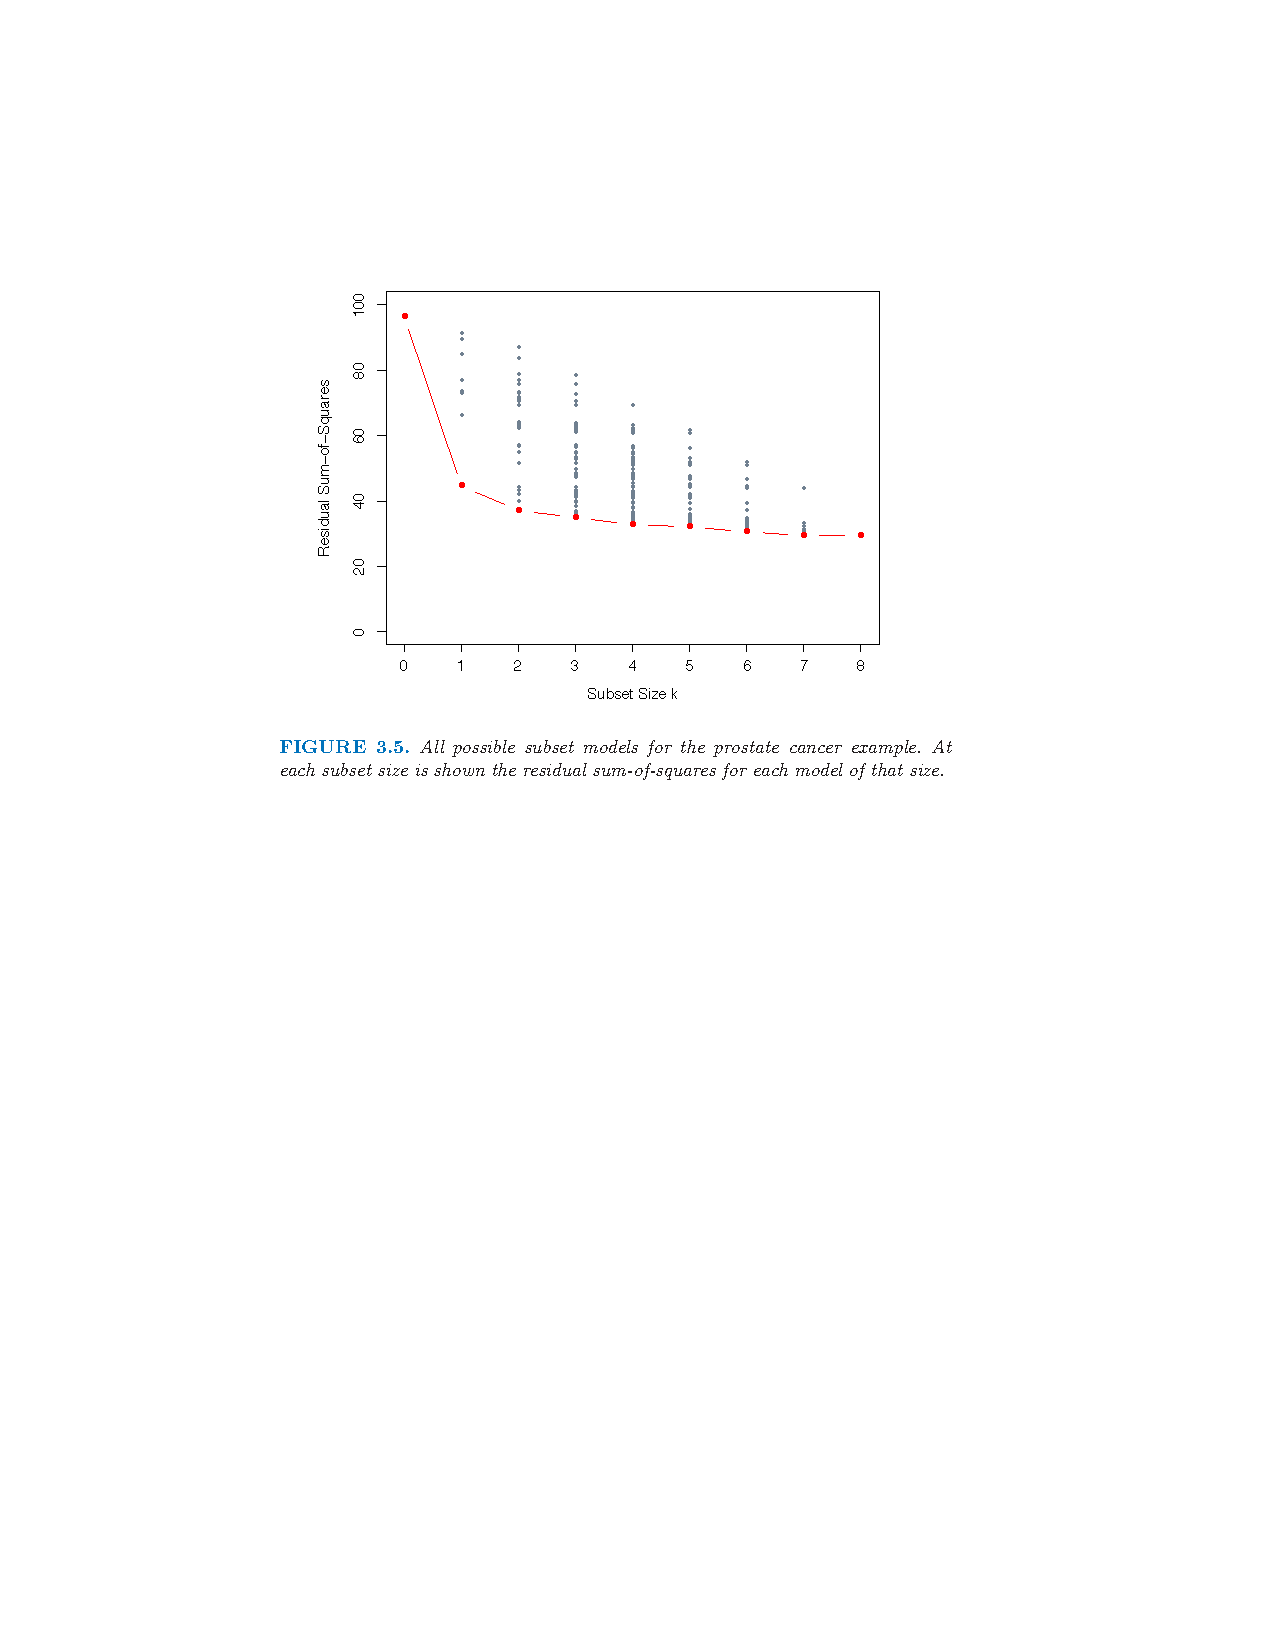
\includegraphics[width=\textwidth]{./resources/subsetsaic}
\end{center}
\end{frame}


\begin{frame}
\frametitle{Forward Stepwise Regression}
Consider the following \alert{greedy algorithm}
\begin{enumerate}
\item Start with an empty model and add a constant $\overline{y}$.
\item Then run $K$ single-variable regressions, choose the $x_k$ with the highest $t$-statistic call this $x^{(1)}$.
\item Now run $K-1$ two variable regressions where the constant and $x^{(1)}$ and choose $x^{(2)}$ as regression where $x_k$ has the highest t-statistic.
\item Now run $K-2$ three variable regressions where the constant and $x^{(1)},x^{(2)}$
\item You get the idea!
\end{enumerate}
We stop when the $x_k$ with the highest t-statistic is below some threshold (often 20\% significance).
\end{frame}


\begin{frame}
\frametitle{Backwards Stepwise Regression}
\begin{enumerate}
\item Start with an full model.
\item Remove the $x$ variable with the lowest $t$-statistic. Call this $x^{(k)}$.
\item Re-run the regression without $x^{(k)}$.
\item Repeat until the smallest $t$-statistic exceeds some threshold.
\end{enumerate}
\end{frame}


\begin{frame}
\frametitle{Comparison}
\begin{itemize}
\item Backwards and fowards stepwise regression tend to give similar choices (but not always).
\item Everything is trivial if $X$'s columns are orthogonal (computer has some tricks otherwise- $QR$).
\item Forward stepwise works when we have more regressors than observations $K > N$.
\item I proposed the $t$-stat here but some packages use AIC/BIC as the criteria.
\item We should also be careful to \alert{group dummy variables together} as a single regressor.
\item These are implemented in \texttt{step} in R and \texttt{stepwise} in Stata.
\item We probably want to adjust our standard errors for the fact that we have run many regressions in sequence before arriving at our model. \alert{In practice not enough people do this!}
\end{itemize}
\end{frame}

\begin{comment}
\begin{frame}
\frametitle{Multiple Testing Problem}
\begin{itemize}
\item A big deal in Econometrics frequently ignored in applied work is the \alert{Multiple Testing Problem}
\item You didn't just pick the regression in your table and run that without considering any others.
\item This means that your $t$ and $F$ stats are going to be too large!! (Standard errors too small!)
\item How much bigger should they be?
\begin{itemize}
\item Analytic size corrections can be tricky and data dependent
\item Bootstrap/Monte-Carlo studies should give you a better idea.
\end{itemize}
\end{itemize}
\end{frame}
\end{comment}


\begin{frame}
\frametitle{(Incremental) Forward Stagewise Regression}
As an alternative consider:
\begin{enumerate}
\item Start with $r= y$ and $(\beta_1, \ldots, \beta_p) = 0$.
\item Find the predictor $x_j$ most correlated with $r$.
\item Update $\beta_j \leftarrow \beta_j + \delta_j$ where $\delta_j = \epsilon \cdot sgn \langle r , x_j \rangle$.
\item Update $r \leftarrow r - \delta_j \cdot x_j$ and repeat for $S$ steps.
\end{enumerate}
\begin{itemize}
\item Alternative $\delta_j =  \langle r , x_j \rangle$
\item We can continue until no regressors have correlation with residuals 
\item This is very slow (it takes many many $S$).
\item Sometimes slowness can be good -- in high dimensions to avoid overfitting.
\end{itemize}
\end{frame}



\begin{frame}
\frametitle{Stepwise selection proedures}
\begin{center}
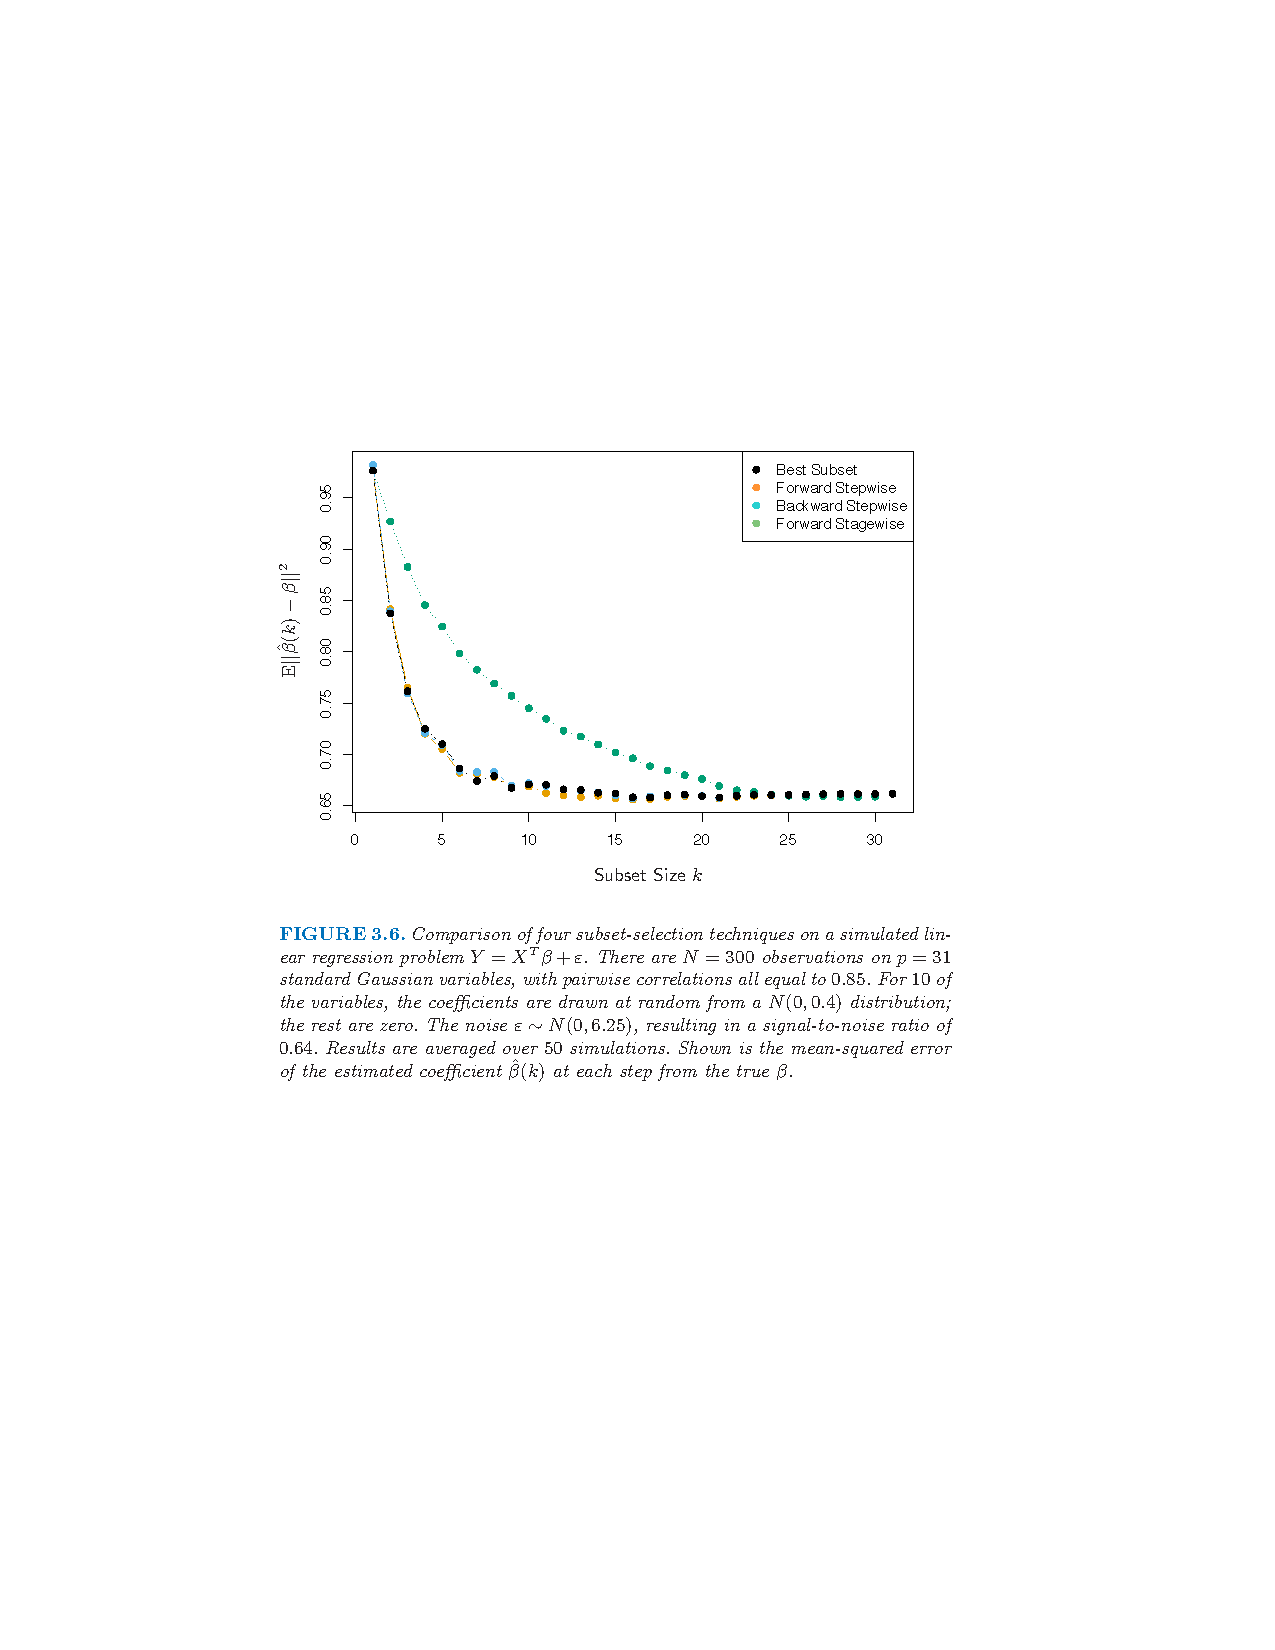
\includegraphics[width=3.5in]{./resources/subsetstepwise}
\end{center}
\end{frame}

\section{Shrinkage}

\begin{frame}
\frametitle{Penalized Regression}
Suppose we fit a regression model and penalized extra variables all in one go, what would that look like?
\begin{eqnarray*}
\hat{\beta} = \arg \min_{\beta} \left[\frac{1}{2} \sum_{i=1}^N (y_i - \beta_0 - \sum_{j=1}^p x_{ij} \beta_j)^2 + \lambda \sum_{j=1}^p | \beta_j|^{q} \right]
\end{eqnarray*}
\begin{itemize}
\item We can consider the penalty term $\lambda \sum_{j=1}^p | \beta_j|^{q}$ as penalizing models where $\beta$ gets further away from zero.
\item Similar to placing a \alert{prior distribution} on $\beta_j$ centered at 0.
\item We definitely want to \alert{standardize} our inputs before using penalized regression methods.
\item Usually you fix $q$ and then look at how estimates respond to $\gamma$.
\item There are two famous cases $q=1$ (Lasso) and $q=2$ (Ridge) though in practice there are many possibilities.
\end{itemize}
\end{frame}


\begin{frame}
    \frametitle{Ridge Regression}
    Another popular alternative is the $q=2$ case
    \begin{eqnarray*}
    \hat{\beta}^{Ridge} = \arg \min_{\beta} \left[\frac{1}{2} \sum_{i=1}^N (y_i - \beta_0 - \sum_{j=1}^K x_{ij} \beta_j)^2 + \lambda \sum_{j=1}^K | \beta_j|^2 \right]
    \end{eqnarray*}
    \begin{itemize}
    \item Penalty is $L_2$ norm on $\beta$.
    \item Can re-write as a constriant  $\sum_{j=1}^K | \beta_j|^2 \leq s$
    \item $\hat{\beta}^{Ridge} = (X'X + \lambda I )^{-1} X' Y$.
    \item If $X$ is orthonormal then $\hat{\beta}_{j}^{Ridge} =  \hat{\beta}_j /(1 +\lambda )$
    \item In words: everything gets dampened by a constant factor $\lambda$ (we don't get zeros).
    \item Adding a constant to the diagonal of $(X'X)$ ensures that the matrix will be invertible even when we have multicollinearity.
    \end{itemize}
\end{frame}

\begin{frame}
    \frametitle{What is rigde doing?}
    \begin{itemize}
        \item Consider the \alert{singular value decomposition} (SVD) on the \textbf{centered} input matrix $$\mathbf{X=UDV^T}$$
        \item \textbf{U} and \textbf{U} are $N \times p$ and $p \times p$ orthogonal matrices spanning the column and rowpace of \textbf{X}. 
        \item \textbf{D} is a $p \times p$ diagonal matrix with $d_1 > d_2 ...d_p > 0$. 
        \item Can see that ols is $$ \mathbf{X} \hat\beta^{LS} = \mathbf{UU^Ty} $$
        \item Then ridge is $$\mathbf{X}\hat\beta^{ridge} = \sum_{j=1}^p \mathbf{u_j}\frac{d_j^2}{d_j^2 + \lambda}\mathbf{u_j^Ty} $$
     \end{itemize}
\end{frame} 

\begin{frame}
    \frametitle{What is rigde doing? II}
    \begin{itemize}
        \item Ridge is shrinking the OLS cordinates of y by $d_j^2/(d_j^2 + \lambda)$
        \item This will have the biggest impact on small $d_j$. What does that mean? 
        \item Consider the sampler variance $\mathbf{X=X^TX/N}$ 
        \item It has eigen decomposition $\mathbf{X^TX = VD^2V^T}$, and the eigenvectors $v_j$ are the \alert{principal components} directions of $X$. 
        \item So this is telling use the ridge is placing more weight on  
     \end{itemize}
\end{frame} 

\begin{frame}
    \frametitle{Ridge Path}
    \begin{center}
    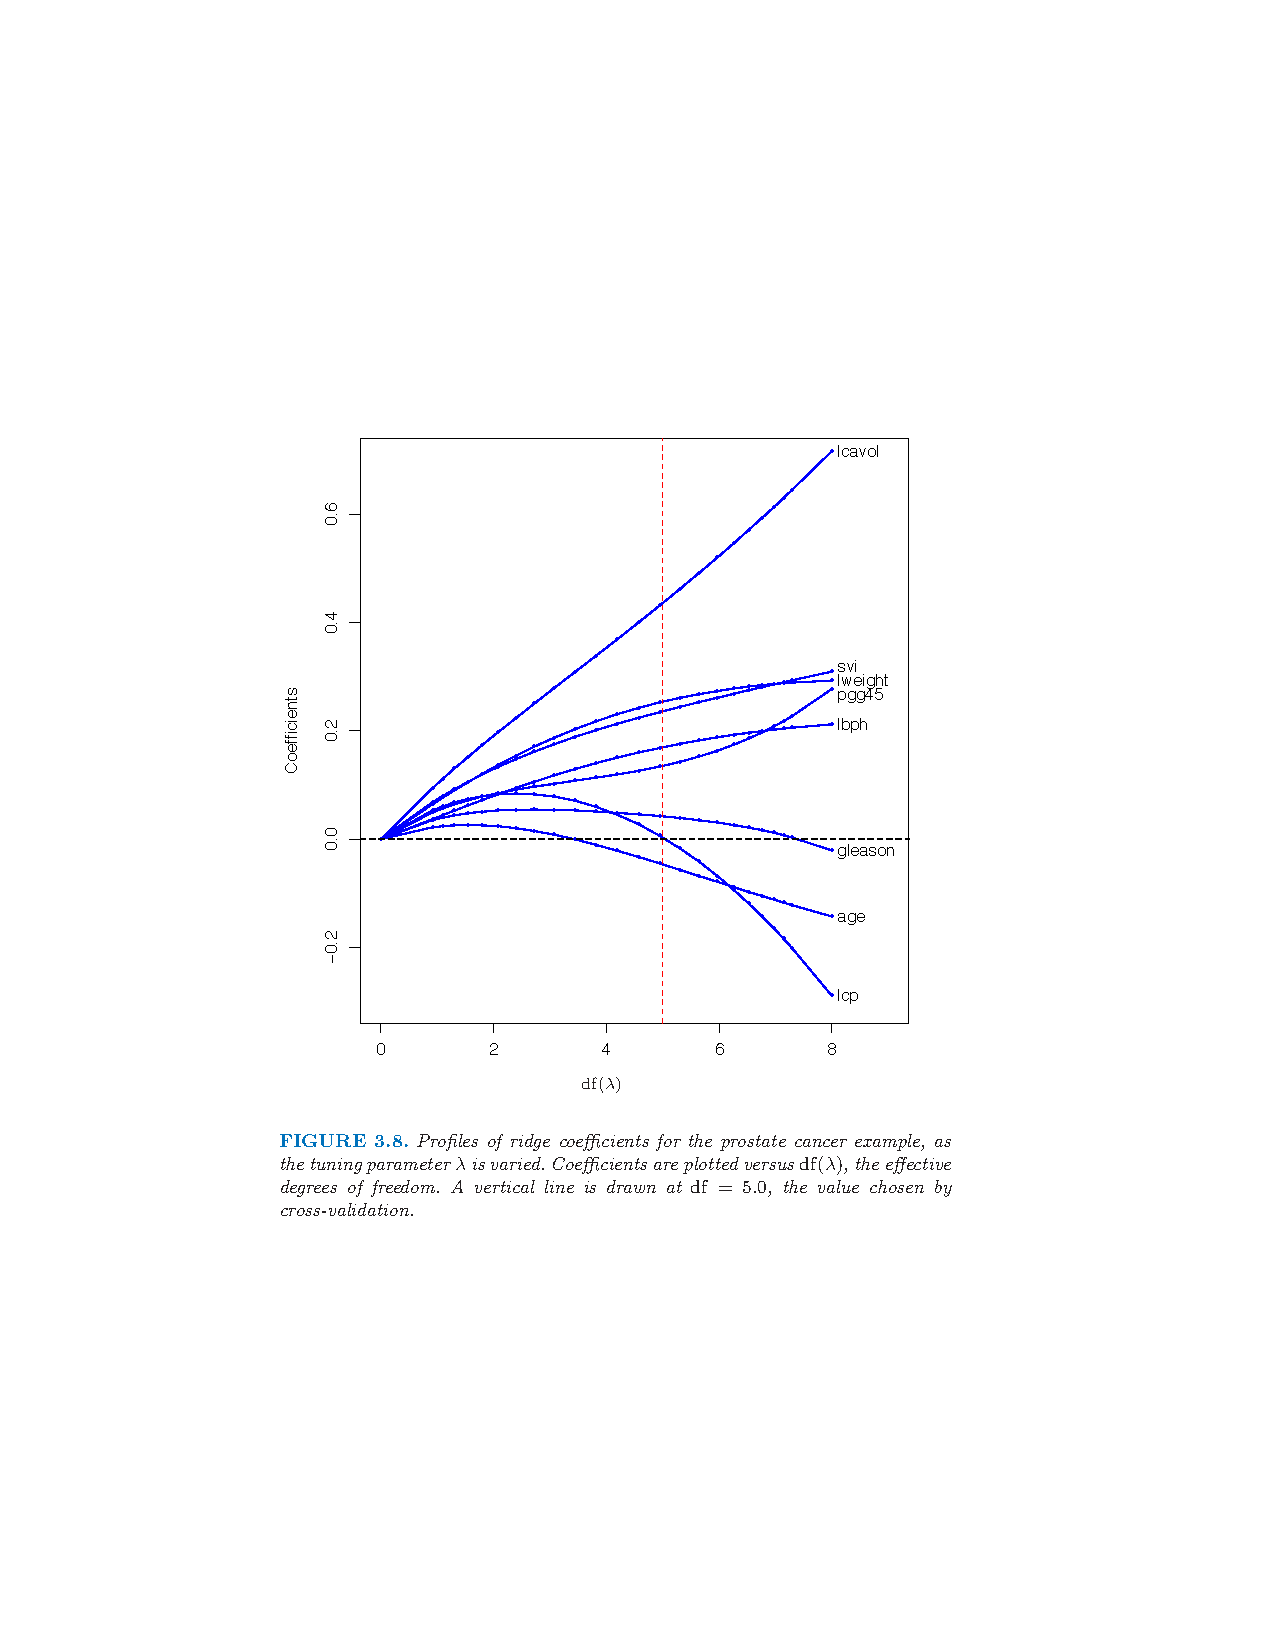
\includegraphics[width=3.5in]{./resources/ridgepath}
    \end{center}
\end{frame}
    
\begin{frame}
\frametitle{LASSO Regression}
\begin{eqnarray*}
\hat{\beta}^{LASSO} = \arg \min_{\beta} \left[\frac{1}{2} \sum_{i=1}^N (y_i - \beta_0 - \sum_{j=1}^K x_{ij} \beta_j)^2 + \lambda \sum_{j=1}^K | \beta_j| \right]
\end{eqnarray*}
\begin{itemize}
\item Penalty is $L_1$ norm on $\beta$.
\item Can re-write as a constriant  $\sum_{j=1}^K | \beta_j| \leq s$
\item If $X$ is orthonormal then $\hat{\beta}_{j}^{LASSO} = sign(\hat{\beta}_j ) \cdot (| \hat{\beta}_j |- \lambda )_{+}$
\item In words: we get coefficients that are closer to zero by $\lambda$, but coefficients within $\lambda$ of zero are shrunk to zero.
\item This leads people to describe LASSO as a \alert{shrinkage} estimator. It produces models that are \alert{sparse}.
\item Instead of a discrete parameter such as the number of lags $p$ we can continuously penalize additional complexity with $\lambda$.
\end{itemize}
\end{frame}


\begin{frame}
\frametitle{LASSO Regression}
But... is choosing $\lambda$ any easier than choosing $p$?
\begin{itemize}
\item We call $\lambda$ the \alert{regularization} parameter.
\item We can choose $\lambda$ in a way that minimizes expected prediction error (EPE).
\item Recall $EPE(\lambda) = E_x E_{y|x} ([ Y- g(X,\lambda)]^2 | X)$.
\item In practice most people look at out of sample prediction error rate on a \alert{cross validated sample}.
\end{itemize}
\end{frame}

\begin{frame}
\frametitle{LASSO Path}
\begin{center}
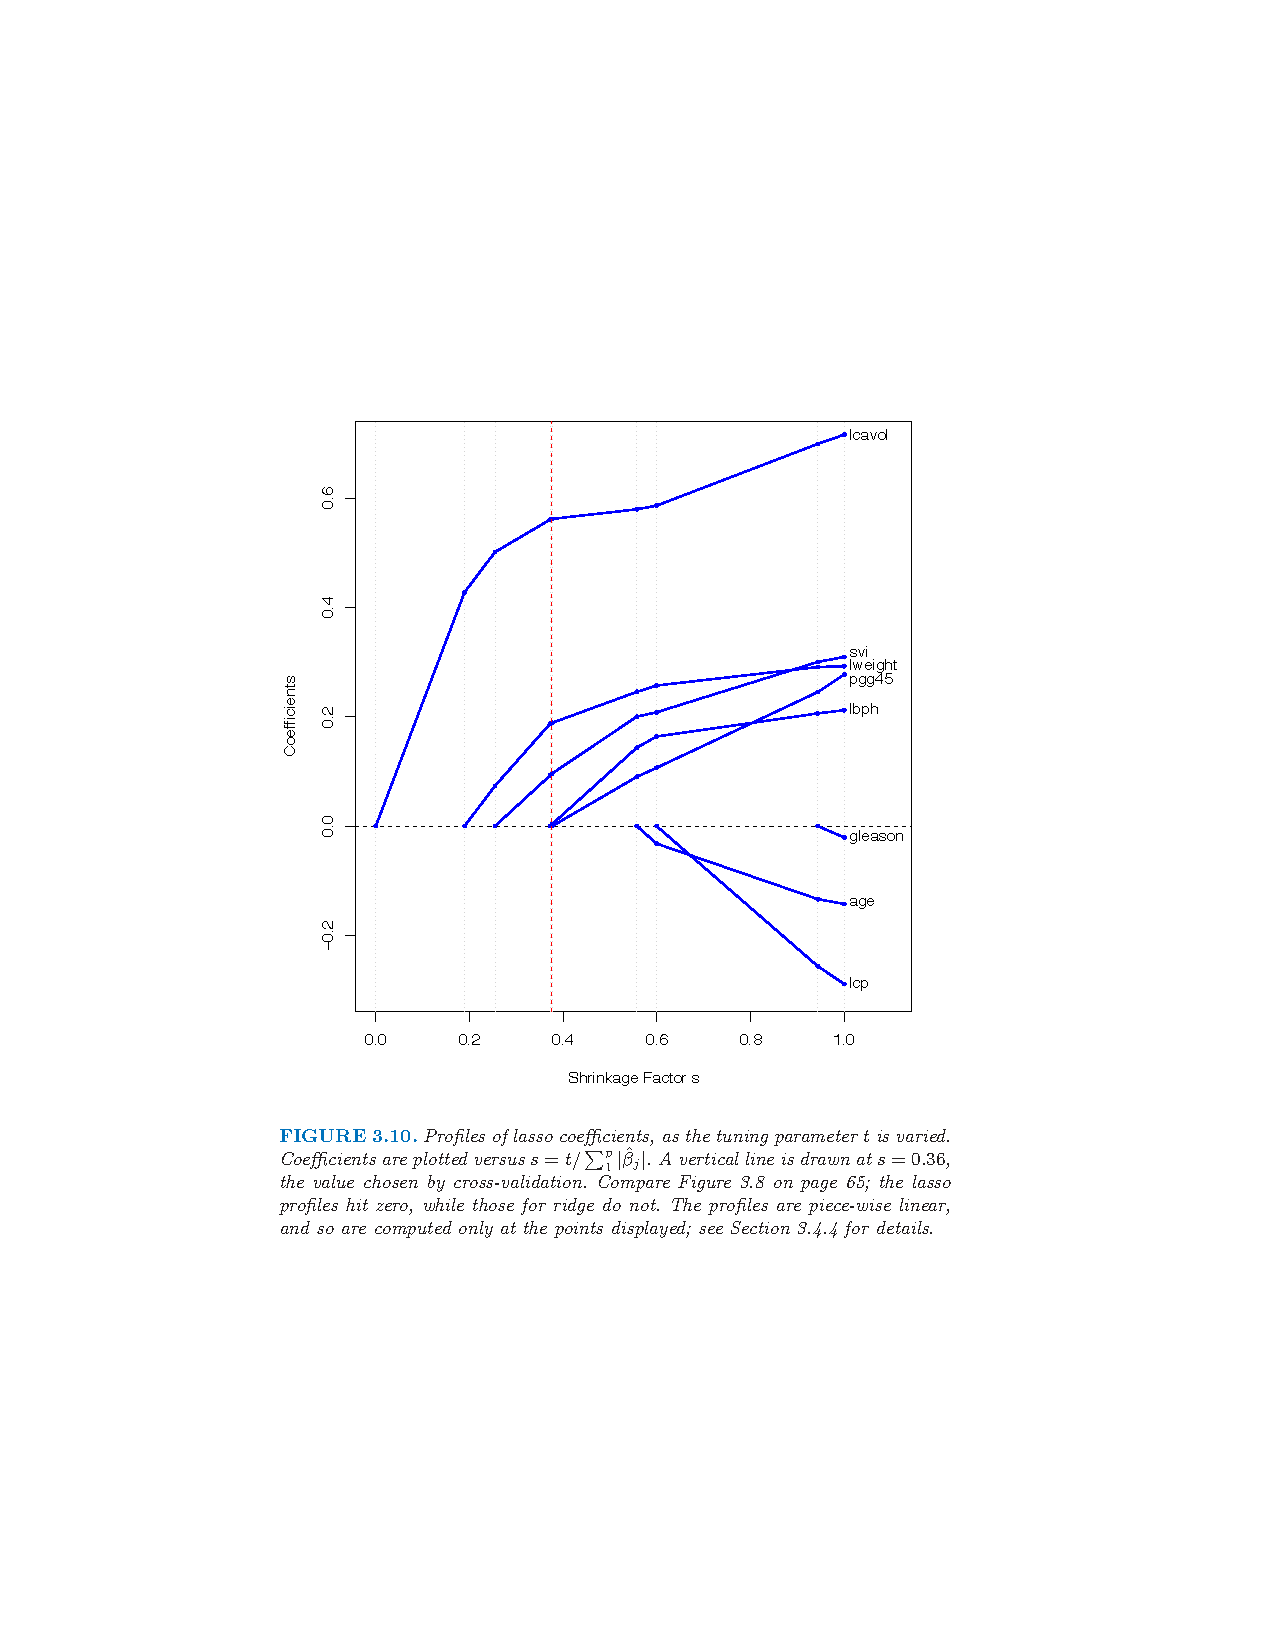
\includegraphics[width=3.5in]{./resources/lassopath}
\end{center}
\end{frame}

\begin{frame}
\frametitle{LASSO vs Ridge}
\begin{center}
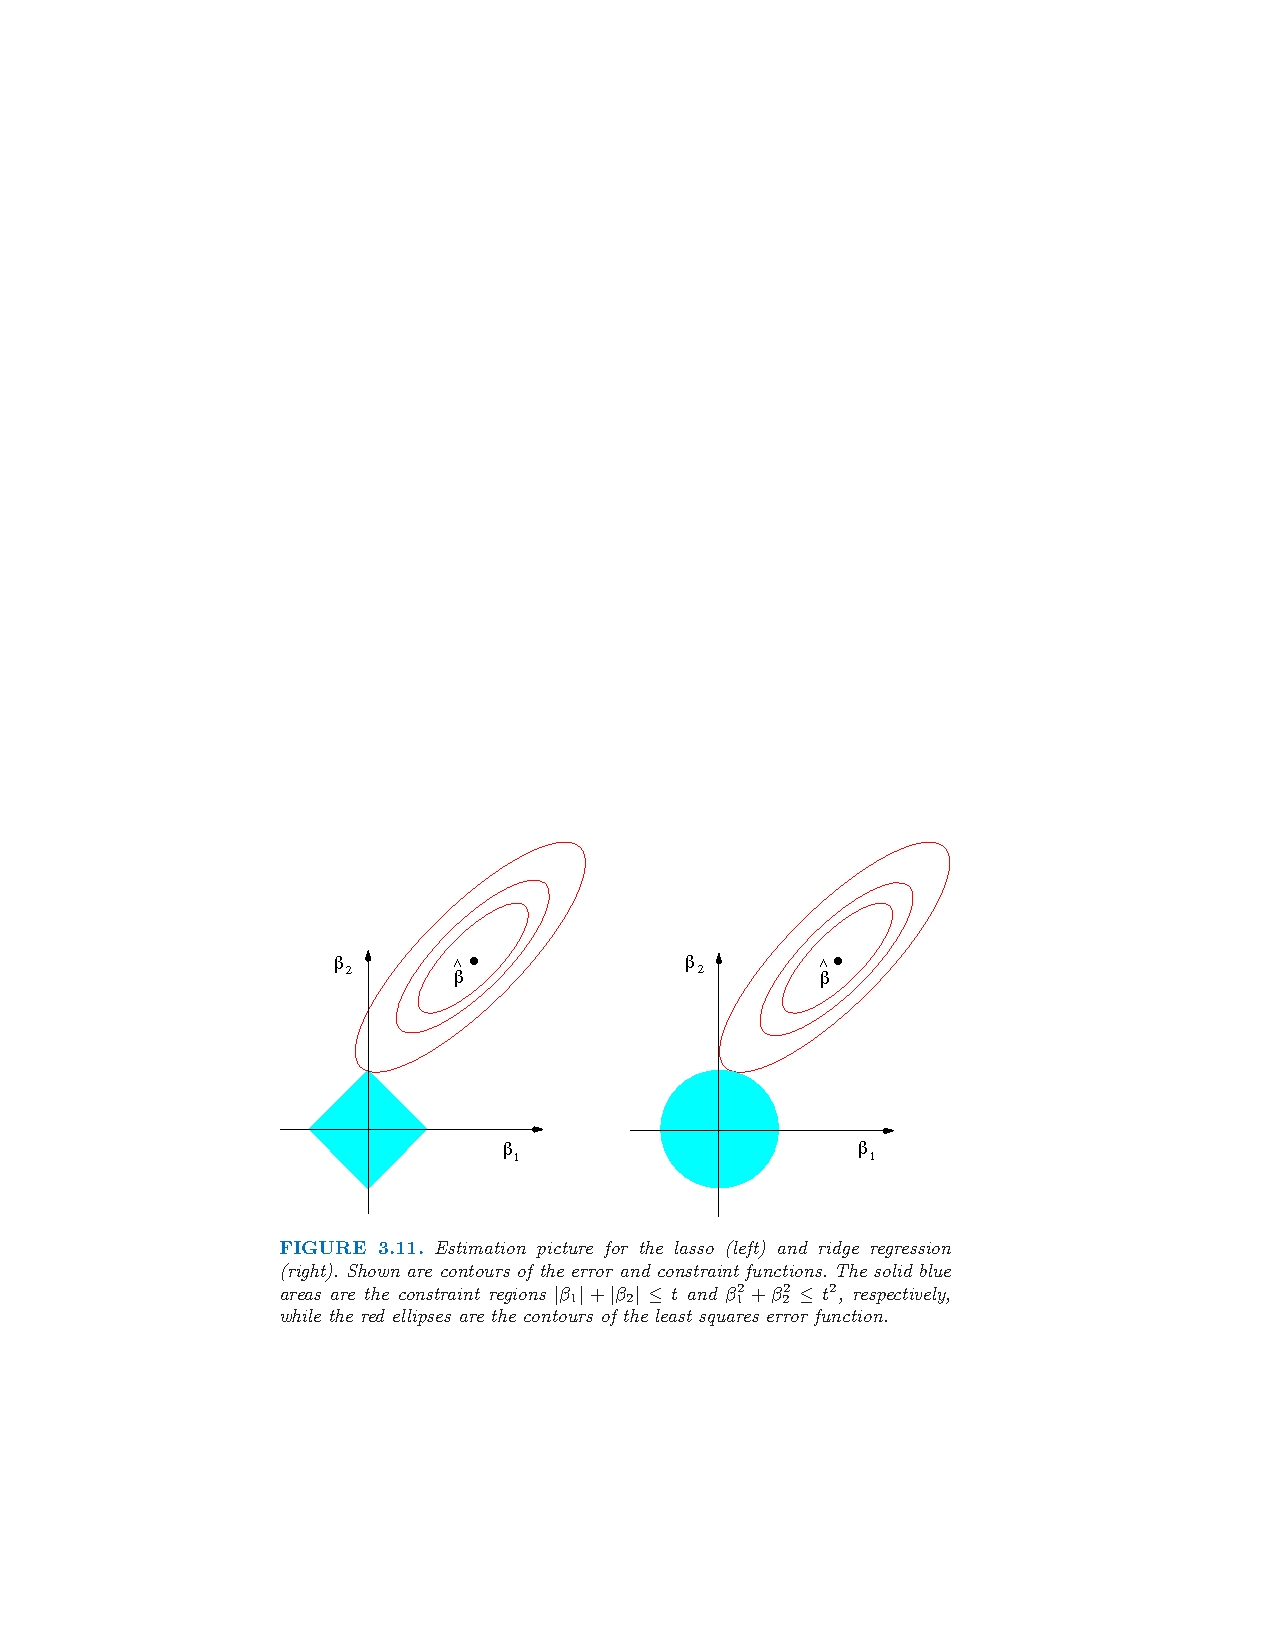
\includegraphics[width=3.5in]{./resources/geometry}
\end{center}
\end{frame}

\begin{frame}
\frametitle{What is the point?}
Ridge:
\begin{itemize}
\item Ridge doesn't provide sparsity which can be a good thing.
\item It is most helpful (relative to OLS) when $X$'s are highly correlated with one another.
\item OLS can set large but imprecise coefficients when it cannot disentangle effects.
\end{itemize}
LASSO:
\begin{itemize}
\item LASSO is useful for variable/feature selection.
\item LASSO does not generally posses the \alert{oracle property} though variants such as \alert{adaptive LASSO} may.
\item LASSO sometimes has the oracle property for $p \gg N$ and cases where the true $\beta$'s are not too large.
\item People sometimes use LASSO to choose components and then OLS for unbiased coefficient estimated.
\end{itemize}
We can actually combine them using \alert{elastic net regression}:
\begin{eqnarray*}
 P(\lambda_1,\lambda_2,\mathbf{\beta}) =  \lambda _1\sum_{j=1}^K | \beta_j|  +\lambda_2 \sum_{j=1}^K | \beta_j|^2 
 \end{eqnarray*}
\end{frame}


\begin{frame}
\frametitle{LASSO vs. Ridge}
\begin{center}
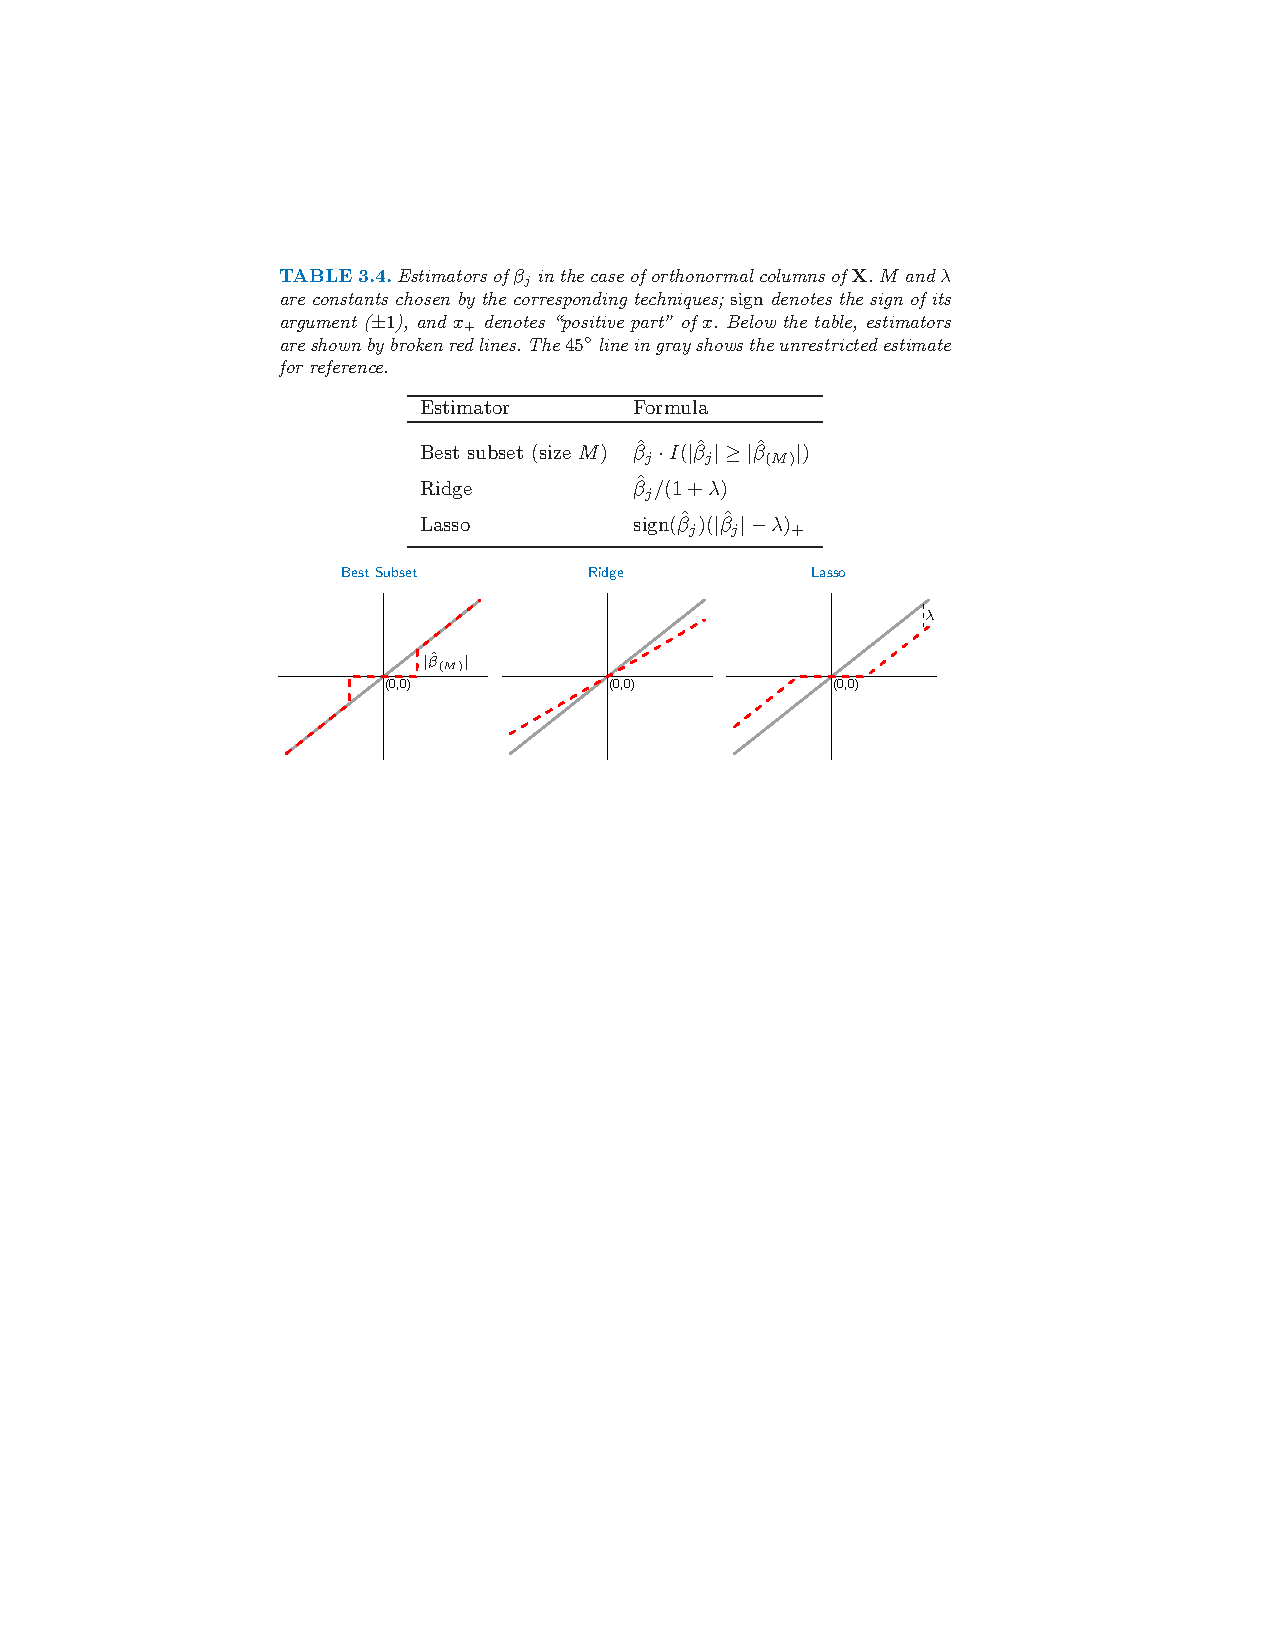
\includegraphics[width=3.5in]{./resources/orthcompare}
\end{center}
\end{frame}


\begin{frame}
\frametitle{LAR: Least Angle Regression}
Remember Forward Stagewise Regression, consider this alternative:
\begin{enumerate}
\item Start with $r= y-\overline{y}$ and $(\beta_1, \ldots, \beta_p) = 0$. (Standardize first!)
\item Find the predictor $x_j$ most correlated with $r$.
\item Move $\beta_j$ from 0 to its least-squares estimate $\langle<x_j , r \rangle$ slowly
\item Update $r \leftarrow r - \delta_j \cdot x_j$.
\item Keep moving $x_j$ in same direction until $x_k$ has as much correlation with updated $r$,
\item Continue updating $(\beta_j, \beta_k)$ in direction of \alert{joint} least-squares coefficients until some other competitor $x_l$ has as much correlation with $r$.
\item Continue until all $p$ predictors have entered. After $\min[N-1,p]$ steps we arrive at full OLS solution.
\end{enumerate}
\begin{itemize}
\item \alert{Optional:} If a current least-squares estimate hits zero drop it from the active set and re-estimate the joint least squares direction without it.
\end{itemize}
\end{frame}


\begin{frame}
\frametitle{LAR: Least Angle Regression}
Why do we need LAR?
\begin{itemize}
\item It turns out that with the optional step from the previous slide: LAR gives us an easy algorithm to compute the LASSO estimate.
\item Actually it does even better -- it gives us the full path of LASSO estimates for all values of $\lambda$!
\item This is actually a relatively new result.
\end{itemize}
\end{frame}


\begin{frame}
\frametitle{LASSO vs LAR}
\begin{center}
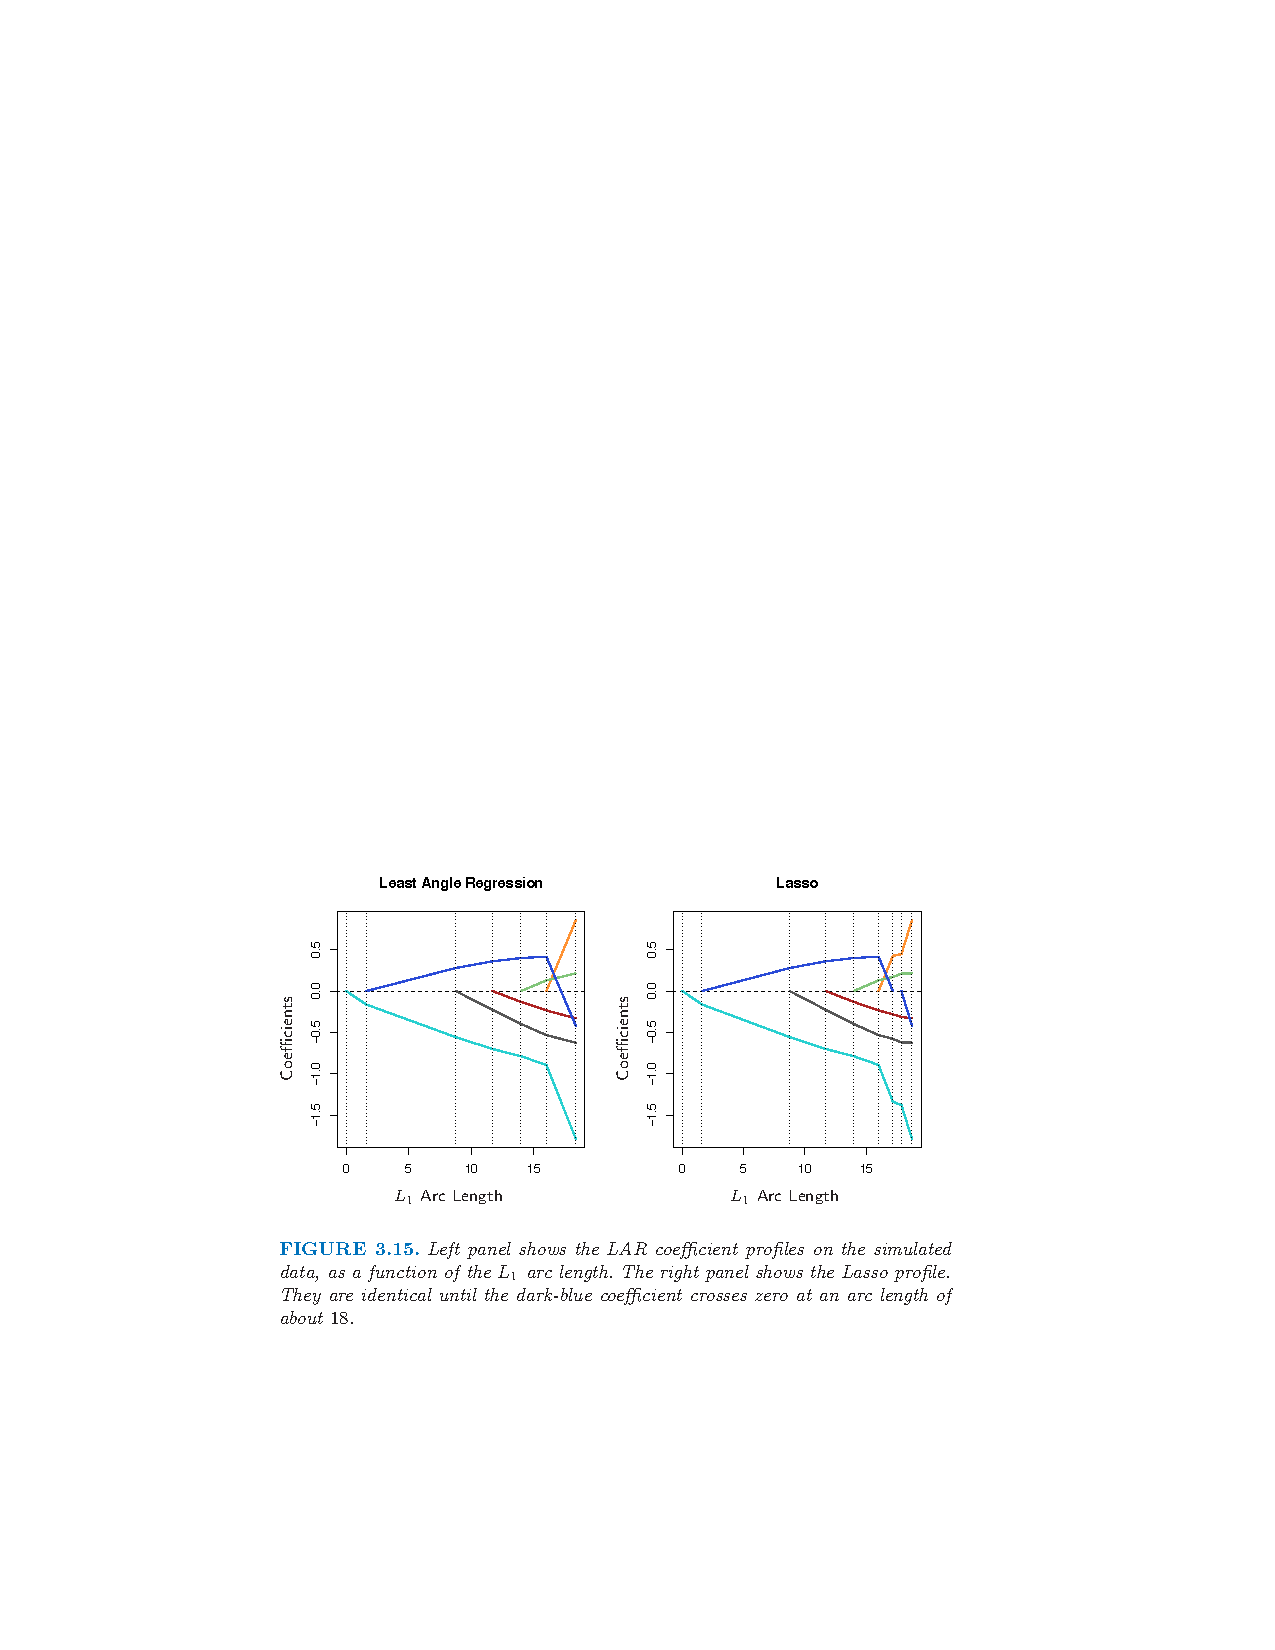
\includegraphics[width=3.5in]{./resources/lar-lasso}
\end{center}
\end{frame}

\begin{frame}
\frametitle{Overall Comparison}
\begin{center}
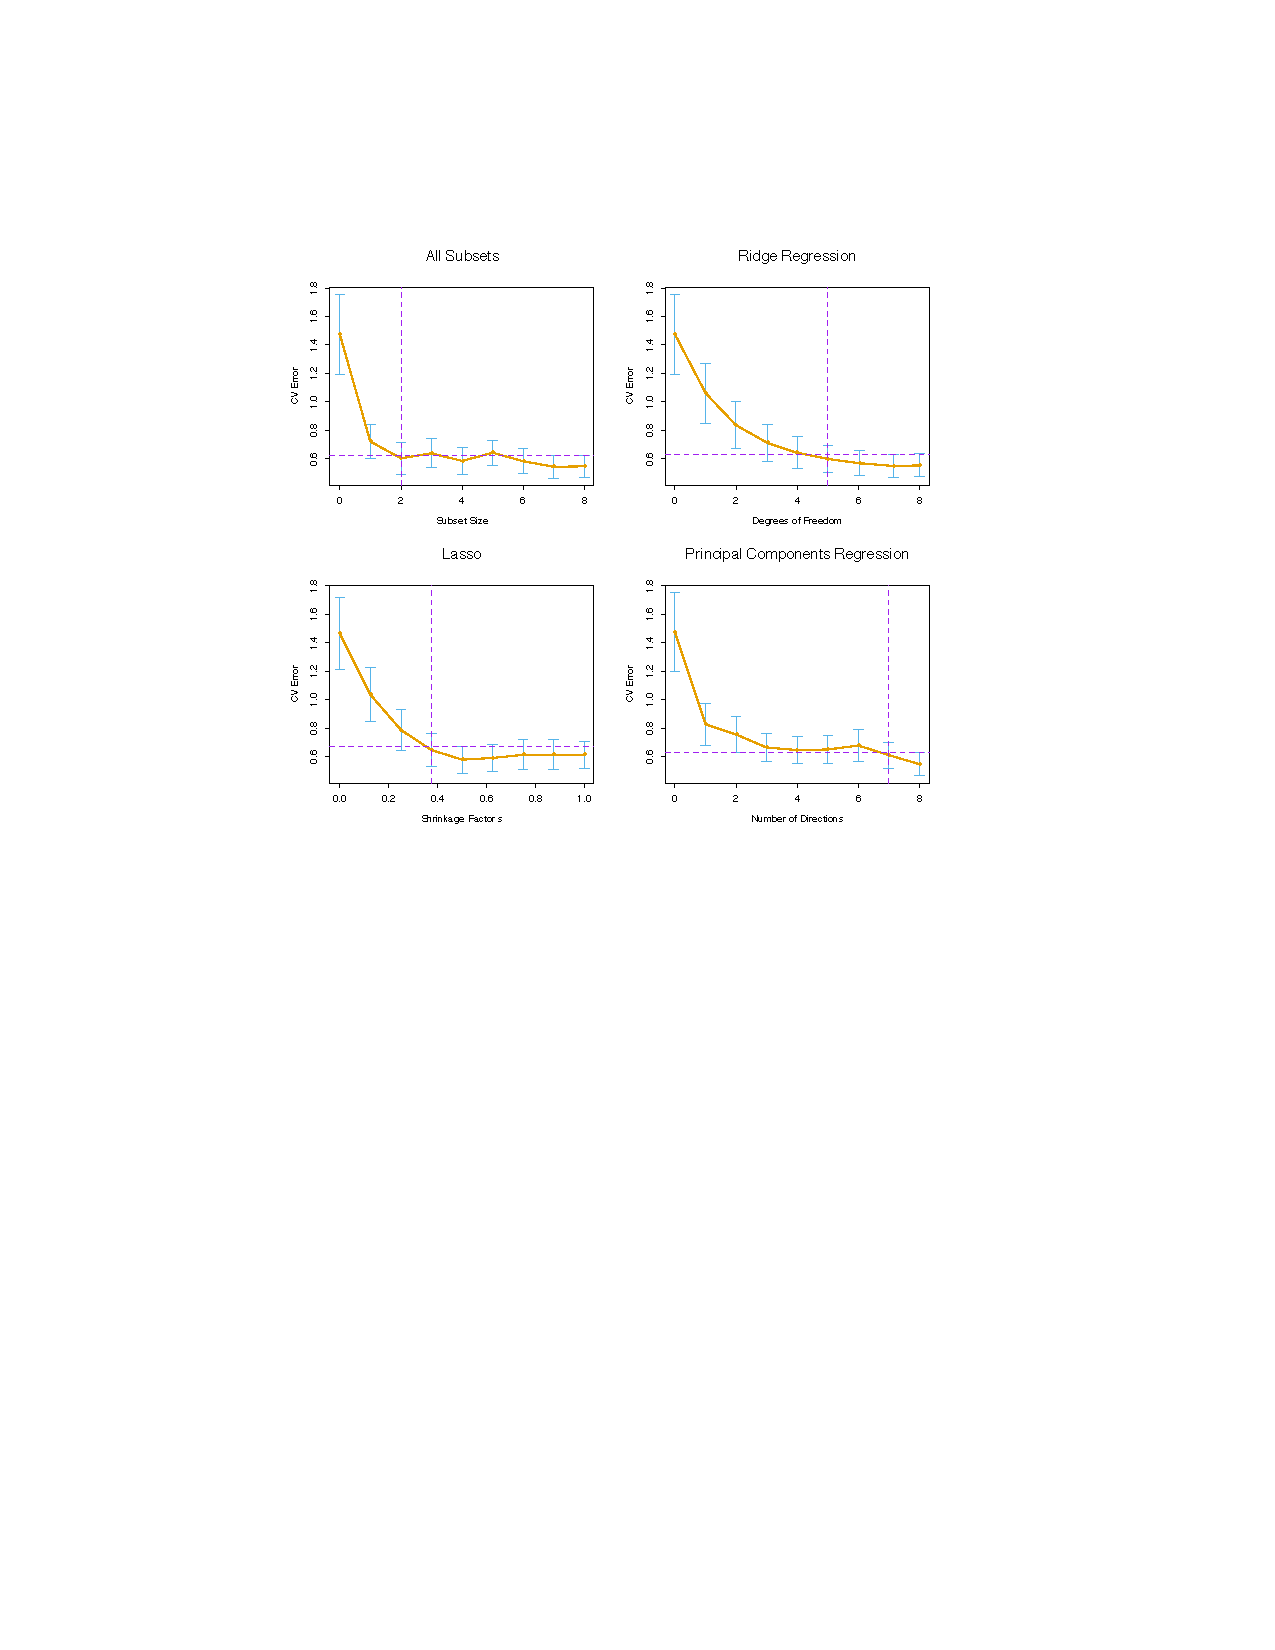
\includegraphics[width=3.5in]{./resources/comparisons}
\end{center}
\end{frame}

\begin{frame}
\frametitle{Overall Comparison}
\begin{center}
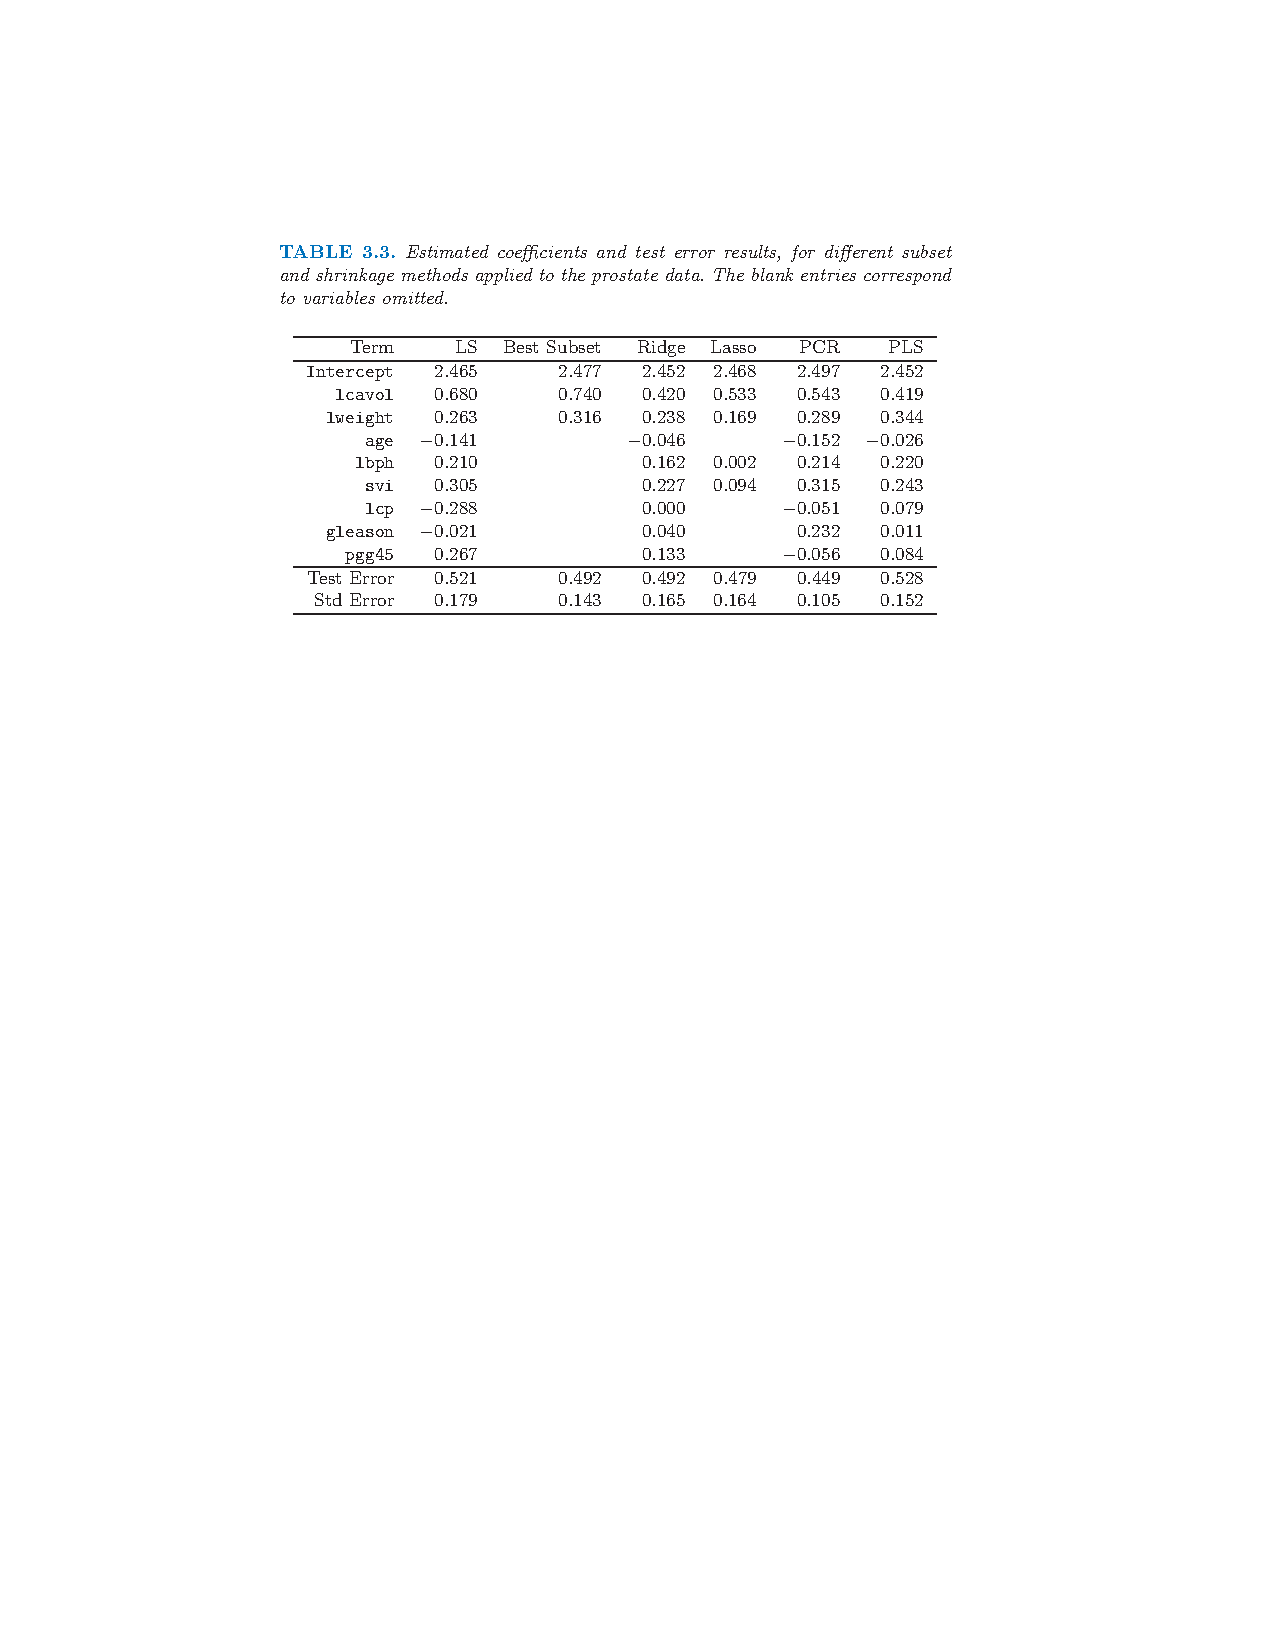
\includegraphics[width=4in]{./resources/regressiontable}
\end{center}
\end{frame}


\begin{frame}
\frametitle{Overall Comparison}
\begin{center}
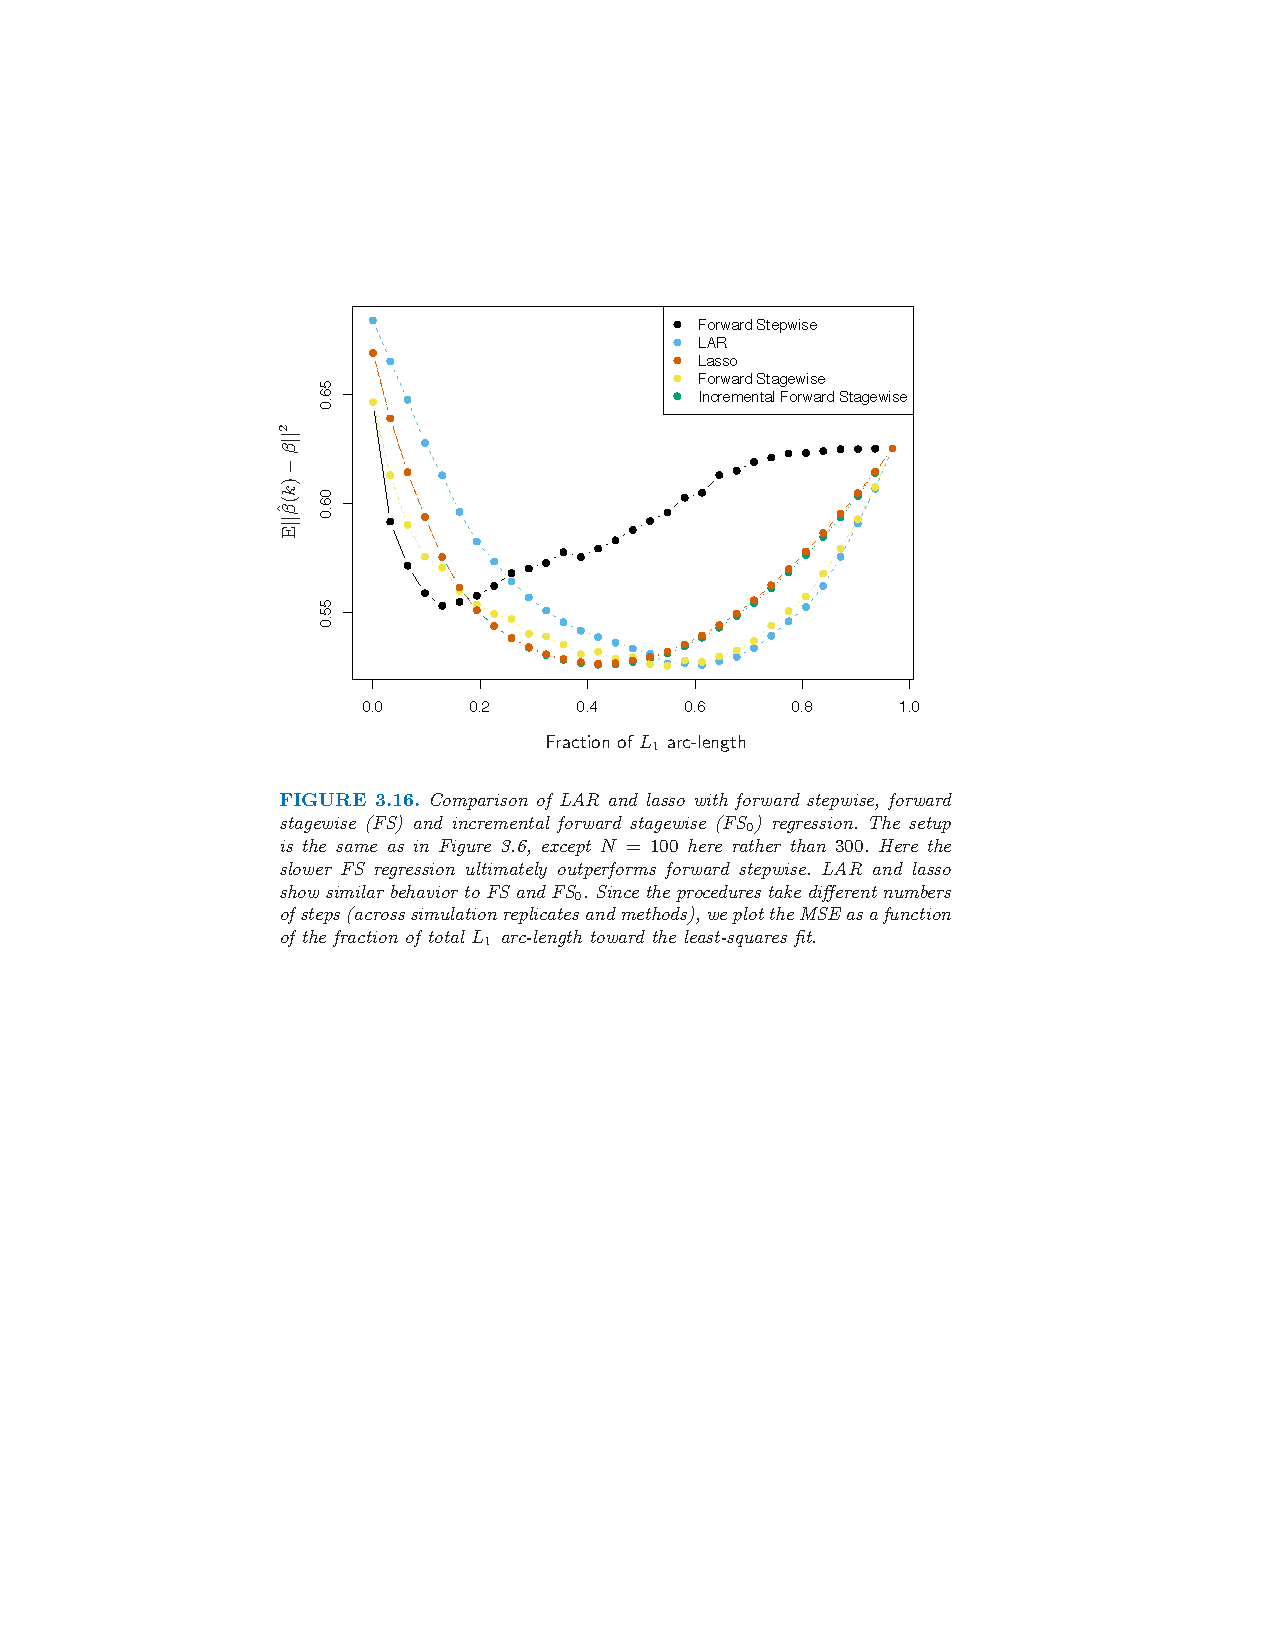
\includegraphics[width=3.5in]{./resources/compareall}
\end{center}
\end{frame}

\begin{frame}
\frametitle{Implementation}
\begin{itemize}
\item Routines are highly specialized: there are lots of tricks
\item No hope of coding this up on your own!
\item In R you can use \texttt{glmnet} or \texttt{lars}.
\item In Python you can use \texttt{scikit-learn}
\item In most recent Matlab in Stats toolbox you have \texttt{lasso} and \texttt{ridge}.
\item In STATA you can download \texttt{.ado} files from Christian Hansen's website (Chicago).
\end{itemize}
\end{frame}

\begin{frame}
\frametitle{Other Data Reduction Techniques}
We have other data reduction techniques with a long history in Econometrics
\begin{itemize}
\item Principal Components
\item Factor Analysis
\item Partial Least Squares
\end{itemize}
\end{frame}

\begin{frame}
\frametitle{Principal Components}
Suppose we have a very high dimensional $X$ where we have a high degree of correlation among the components $x_j$. 
\begin{itemize}
\item We can start by computing the appropriate correlation matrix $C=E[\tilde{X}'\tilde{X}]$ where $\tilde{X}$ denotes we have standardized each column $x_j$ to have mean zero and variance 1.
\item Diagonlize $C$ via the eigen-decomposition $V^{-1} C V = D$ where $D$ is the diagonal matrix of eigenvalues.
\item Sort $D$ and the corresponding columns of $V$ in decreasing order of the eigenvalues $d_j$.
\item Choose a subset of $m < K$ eigenvalues and eigenvectors and call that $V_m$ and $\lambda_m$
\item Compute transformed data: $Z_m = V_m \tilde{X}$ which is of dimension $N \times m$ instead of $N \times K$.
\end{itemize}
\end{frame}

\begin{frame}
\frametitle{Principal Components}
\begin{itemize}
\item If $m \ll K$ then we can substantially reduce the dimension of the data.
\item The idea is to choose $m$ so that $(Z'Z)$ spans approximately the same space that $(X'X)$ does.
\item This works because we use the \alert{principal eigenvectors} (those with the largest eigenvalues).
\item The first eigenvector explains most of the variation in the data, the second the most of the remaining variation, and so on.
\item You may also recall that eigenvectors form an \alert{orthonormal basis}, so each dimension is linearly independent of the others.
\item As eigenvalues decline, it means they explain less of the variance.
\end{itemize}
\end{frame}

\begin{frame}
\frametitle{Principal Components}
Output from software will inlcude
\begin{itemize}
\item Coefficients: these transform from $X\rightarrow Z$
\item Score: these are the transformed $Z$'s
\item Latent/Eigenvalue: the corresponding Eigenvalue
\item Explained/Cumulative: cumulative explained variance $ \sum_{j=1}^m( \lambda_j / \sum_k \lambda_k)$
\item Stata: \texttt{pca}, Matlab: \texttt{pca}, R/stats: \texttt{princomp}.
\end{itemize}
\end{frame}

\begin{frame}
\frametitle{Principal Components}
How many components?
\begin{itemize}
\item Choose \# of components by the eigenvalues or \% of variance explained
\item Common cutoffs are 90-95\% of variance.
\item Eigenvalue based cutoff rules (only take eigenvalues $ > 1$).
\item Most common method is to eyeball the scree plot.
\end{itemize}
\end{frame}


\begin{frame}
\frametitle{Principal Components}
\begin{center}
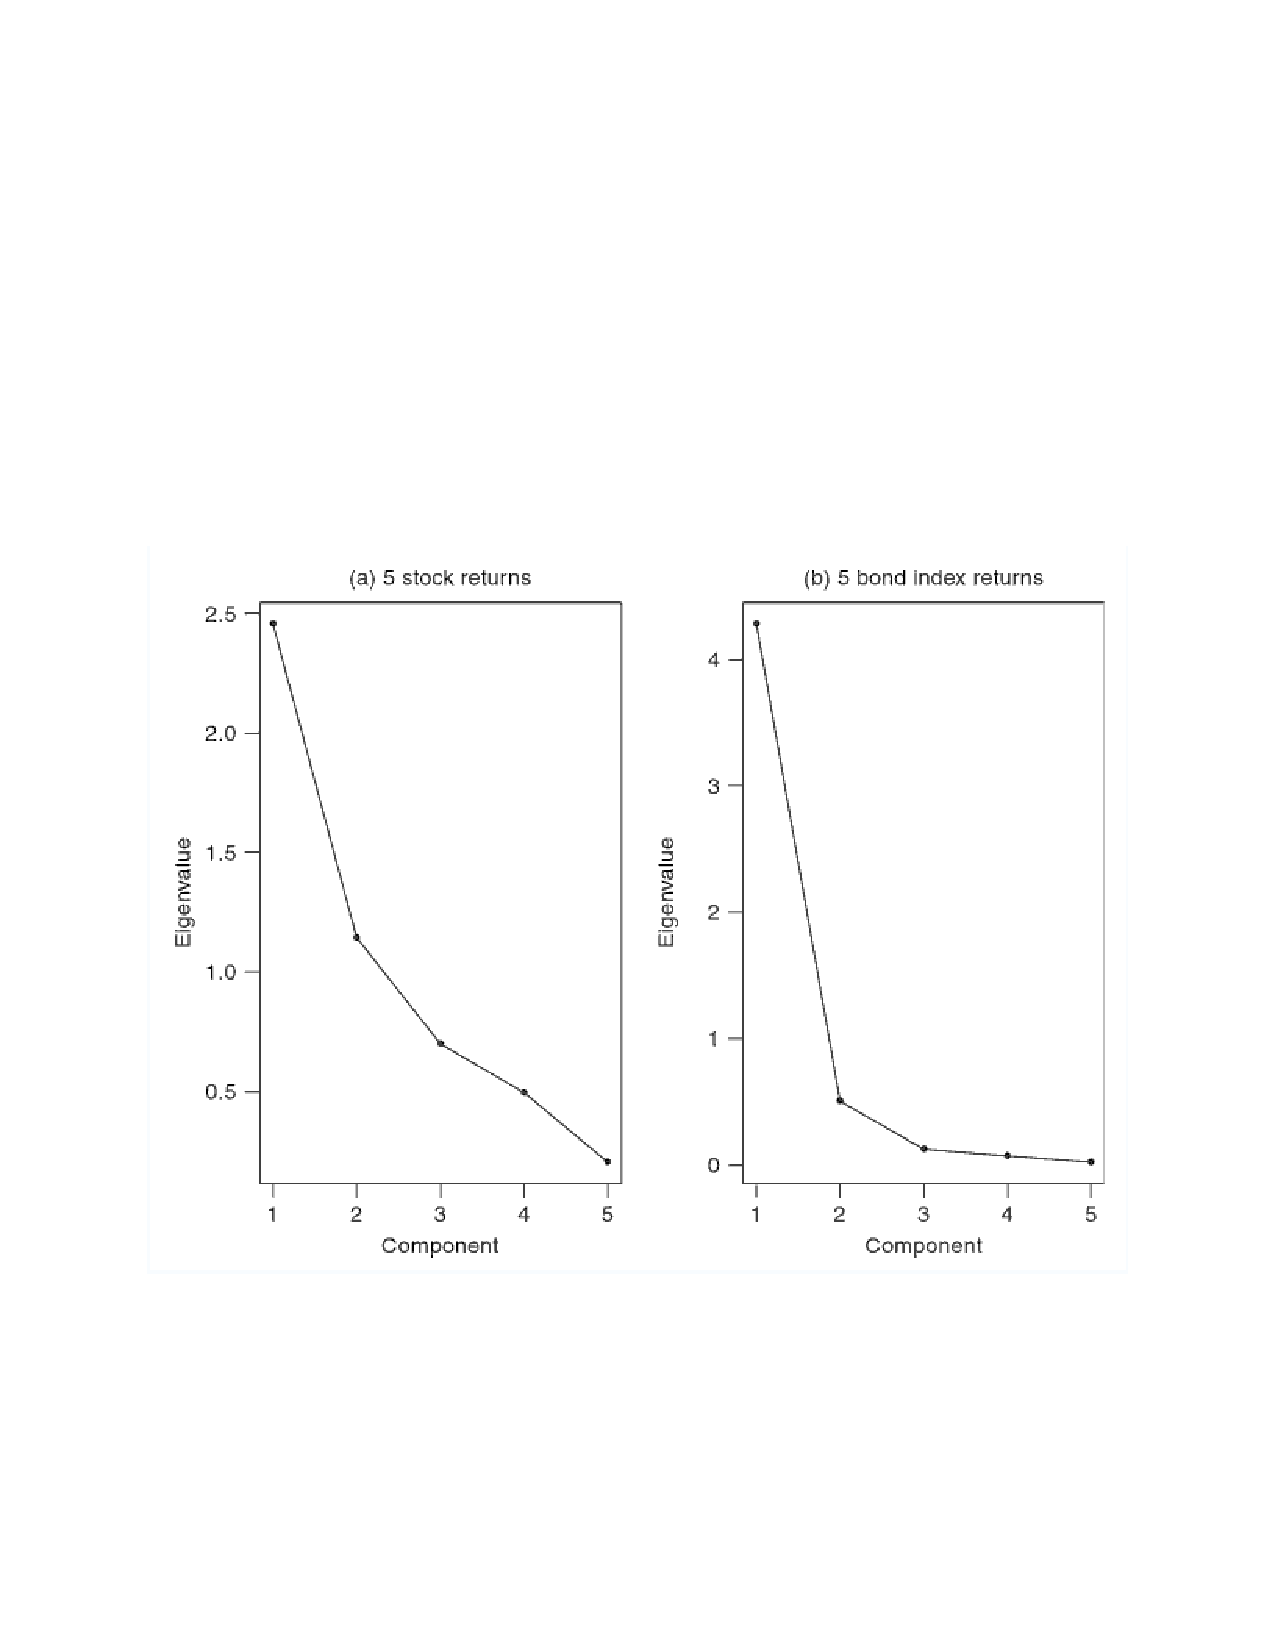
\includegraphics[width=3.5in]{./resources/princomp1}
\end{center}
\end{frame}

\begin{frame}
\frametitle{Principal Components}
\begin{center}
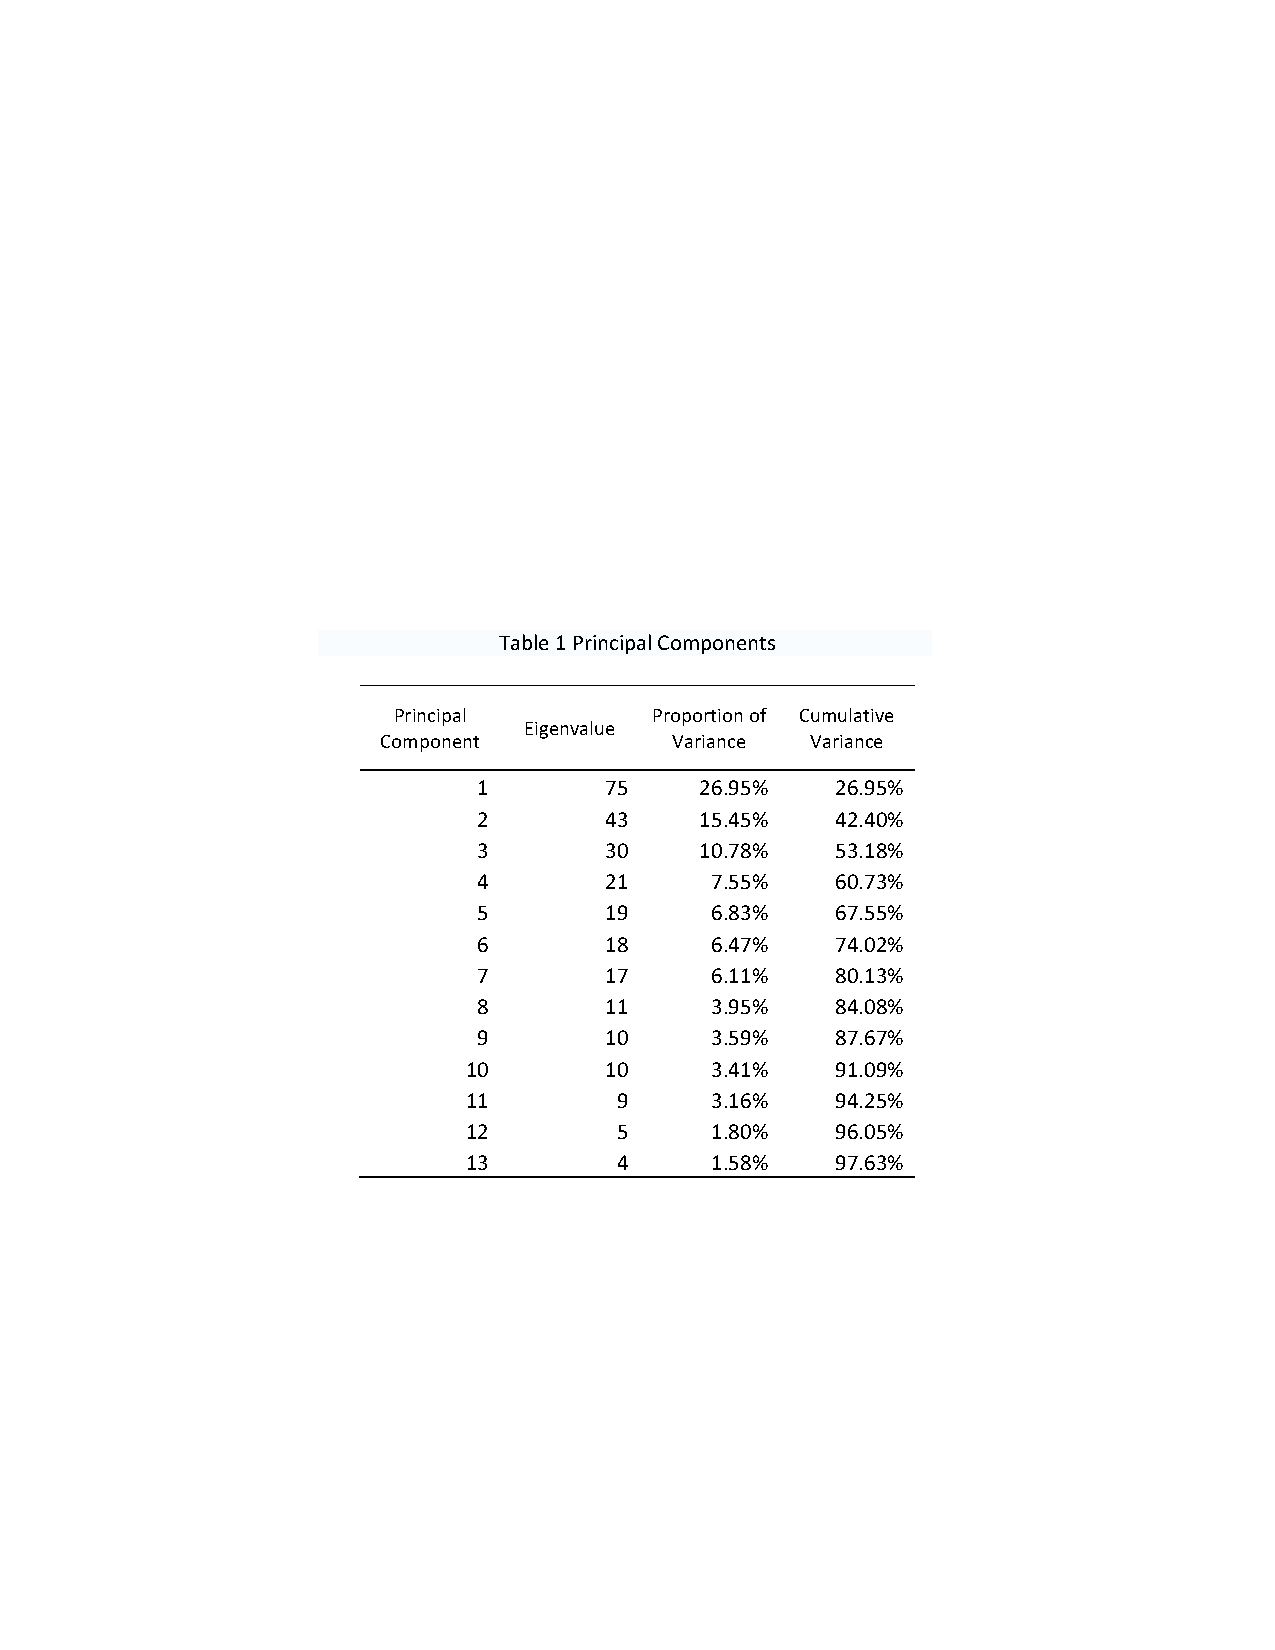
\includegraphics[width=3.5in]{./resources/princomp2}
\end{center}
\end{frame}

\begin{frame}
\frametitle{Principal Components}
\begin{itemize}
\item We can run a regression on principal components $Z$'s and then recover the betas of the $X$'s
\begin{eqnarray*}
\hat{y}_{(M)}^{pcr} = \overline{y} \mathbf{1} + \sum_{m=1}^M \hat{\theta}_m \mathbf{z}_m
\end{eqnarray*}
\item Because principal components are orthogonal we can find coefficients using univariate regression $\hat{\theta}_m = \langle \mathbf{z_m} , \mathbf{y} \rangle / \langle \mathbf{z_m} , \mathbf{z_m} \rangle$.
\item We can recover the $x$ coefficients because the PCA is a linear transformation:
\begin{eqnarray*}
\hat{\beta}^{PCR} = \sum_{m=1}^M \hat{\theta}_m v_m
\end{eqnarray*}
\item If $M=P$ (we use all components) then PCR = OLS.
\item If $M < P$ then we discard the $p-M$ smallest eigenvalue components
\item This is similar to ridge which shrinks $\beta$'s for components with small eigenvalues.
\end{itemize}
\end{frame}
\begin{frame}
\frametitle{Principal Components And Ridge}
\begin{itemize}
\item Think about the variance matrix $X'X/n$ or $X' X = V D^2 V'$.
\item First component (largest eigenvalue) is $\mathbf{z_1} = \mathbf{X} v_1 = \mathbf{u_1} d_1$.
\item Variance is $Var(\mathbf{z_1}) = Var (\mathbf{X} v_1) = \frac{d_1^2}{N}$ ($\mathbf{z_1}$ is first principal component of $\mathbf{X}$).
\end{itemize}
\end{frame}


\begin{frame}
\frametitle{Principal Components}
\begin{center}
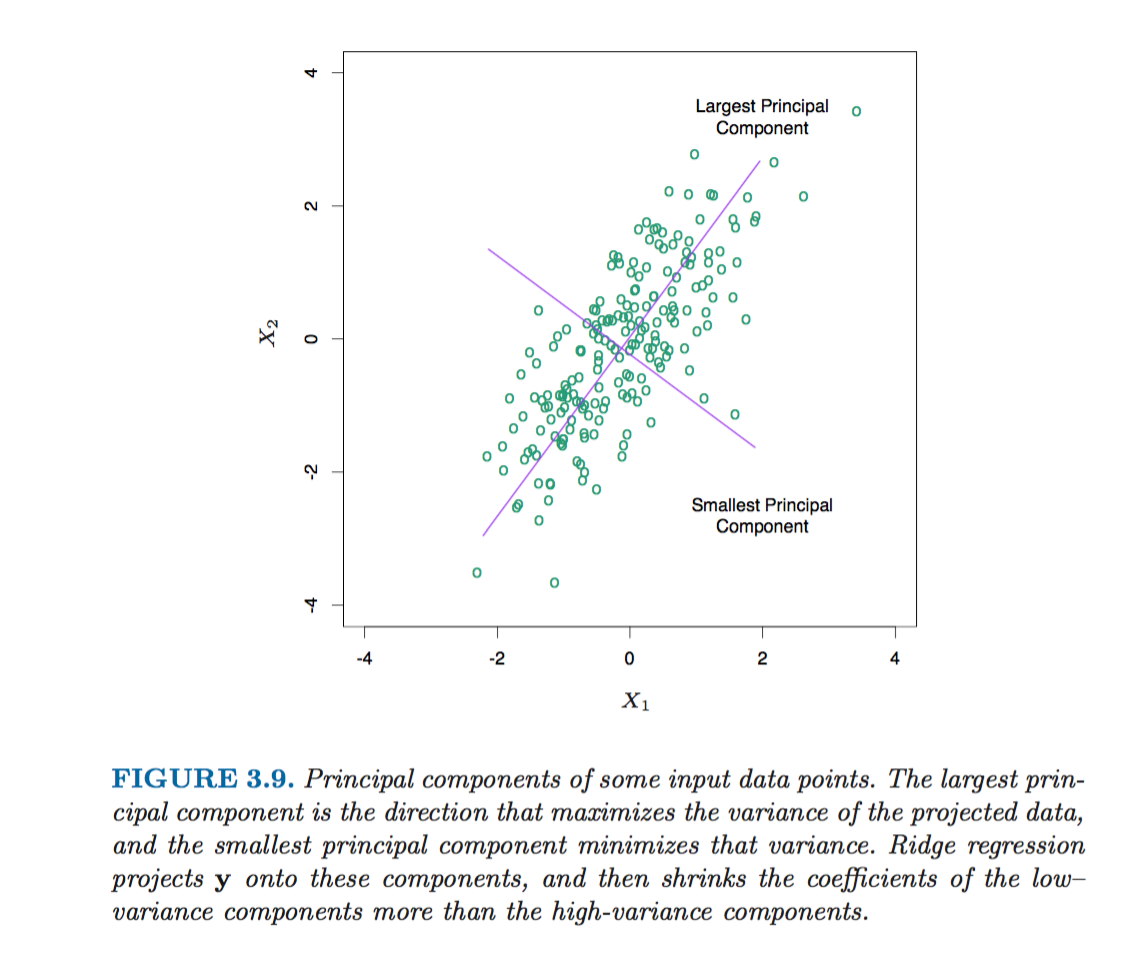
\includegraphics[width=4in]{./resources/princompfig}
\end{center}
\end{frame}




\begin{frame}
\frametitle{Principal Components And Ridge}
Consider the objective function that Ridge minimizes:
\begin{eqnarray*}
RSS(\lambda) = (\mathbf{y} - \mathbf{X} \beta)'  (\mathbf{y} - \mathbf{X} \beta)' + \lambda \beta' \beta
\end{eqnarray*}
And the solution (which addresses multicolinearity!)
\begin{eqnarray*}
\hat{\beta}_{ridge} = (\mathbf{X}' \mathbf{X} + \lambda \mathbf{I})^{-1} \mathbf{X}' \mathbf{y}
\end{eqnarray*}

\end{frame}

\begin{frame}
\frametitle{Principal Components And Ridge}
Just like we can diagonalize (some) square matrices, we can take the \alert{singular value decomposition} (SVD) of any matrix $\mathbf{X}$ that is $N \times p$
\begin{eqnarray*}
\mathbf{X}=\mathbf{U} \mathbf{D} \mathbf{V}'
\end{eqnarray*}
\begin{itemize}
\item $\mathbf{U}, \mathbf{V}$ are $N \times p$ and $p \times p$ orthonormal matrices ($\mathbf{U}$ spans the column space, and $\mathbf{V}$ spans the row space of $X$.)
\item $\mathbf{D}$ is a diagonal matrix $p \times p$ with elements corresponding to the singular values of $\mathbf{X}$.
\item If $\mathbf{X}$ is a square, diagonalizable matrix the singular values are equal to the eigenvalues.
\end{itemize}
\end{frame}

\begin{frame}
\frametitle{Principal Components And Ridge}
Now the least squares solution is simple
\begin{eqnarray*}
\mathbf{X} \hat{\beta}^{ols} = \mathbf{X} (\mathbf{X}'\mathbf{X})^{-1} \mathbf{X}' \mathbf{y} = U U' \mathbf{y}.
\end{eqnarray*}
\begin{itemize}
\item $\mathbf{U}' \mathbf{y}$ are the values of $\mathbf{y}$ mapped into the orthonormal basis $\mathbf{U}$.
\item This looks a lot like $\mathbf{QR}$ except that we have chosen a different basis.
\end{itemize}
Ridge is simple too:
\begin{eqnarray*}
\mathbf{X} \hat{\beta}^{ridge} = \mathbf{X} (\mathbf{X}'\mathbf{X} + \lambda \mathbf{I})^{-1} \mathbf{X}' \mathbf{y} &=& \mathbf{U D} (\mathbf{D}^2 + \lambda \mathbf{I})^{-1} \mathbf{D} \mathbf{U}' \mathbf{y}\\
&=& \sum_{j=1}^p \mathbf{u}_j  \frac{d_j^2}{d_j^2 + \lambda} \mathbf{u}_j' \mathbf{y}
\end{eqnarray*}
\begin{itemize}
\item Same change of basis. Now we shrink each component by $d_j^2/(d_j^2 + \lambda)$.
\end{itemize}
\end{frame}



\begin{frame}
\frametitle{Principal Components}
\begin{center}
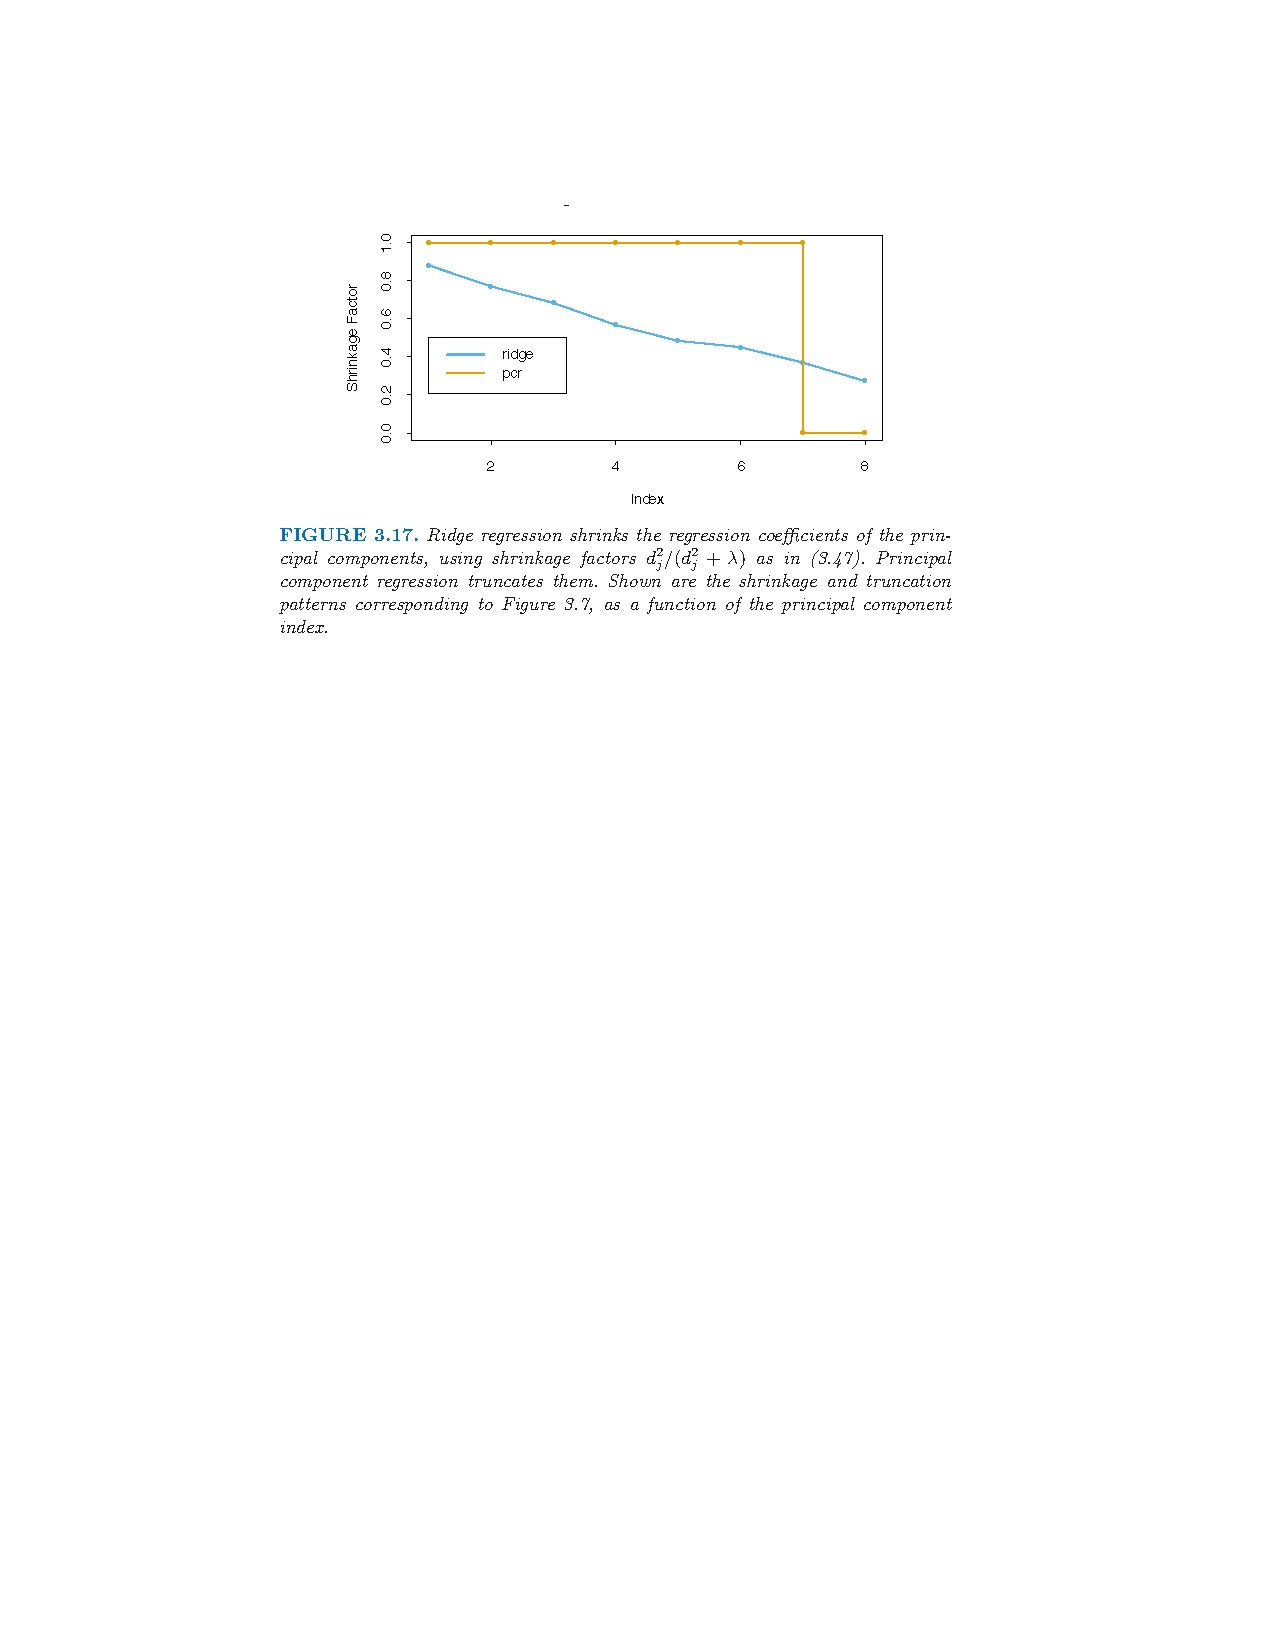
\includegraphics[width=4.5in]{./resources/pcrridge}
\end{center}
\end{frame}



\begin{frame}
\frametitle{Hansen Singleton (1982)}
\begin{itemize}
\item This is the original GMM example, though it comes from macro-finance not microeconometrics
\begin{eqnarray*}
\max_{c_{t+i},A_{t+i}}&& E_t \sum_{i=0}^{\infty} \frac{U(c_{t+i})}{(1+\delta)^i} \quad \mbox{subject to } \\
A_{t+i} &=& (1+r) A_{t+i-1} + y_{t+i} - c_{t+1} \\
0&=&\lim_{i \rightarrow \infty} E_t A_{t+i} (1+r)^{-i} 
\end{eqnarray*}
\item $A_t$ are your investment assets with return $r$ and discount factor $\delta$
\item $y_t$ is your income in period $t$, $c_t$ is your consumption 
\end{itemize}
\end{frame}

\begin{frame}
\frametitle{Hansen Singleton (1982)}
\begin{itemize}
\item Assume CRRA utility with risk aversion $\gamma$
\begin{eqnarray*}
U(c_{t+i})  = \frac{c_{t+i}^{1-\gamma}}{1-\gamma}
\end{eqnarray*}
\item We can take the first-order/Euler conditions and get:
\begin{eqnarray*}
E_t \left(\underbrace{\frac{1+r}{1+\delta} c_{t+1}^{-\gamma} - c_{t}^{-\gamma}}_{g(x_{t+i},\theta)}\right) = 0
\end{eqnarray*}
\item We want to estimate the ``deep parameters'' $\theta \equiv (\gamma,\delta)$.
\end{itemize}
\end{frame}

\begin{frame}
\frametitle{Hansen Singleton (1982)}
\begin{itemize}
\item We can solve for $\theta$ without actually solving the dynamic programming problem!
\item We just need some instruments $z_t$ that are conditionally independent/orthogonal to $g(x_{t+i},\theta)$ so that
\begin{eqnarray*}
E_t [g(x_{t+i},\theta) | z_t] = 0 \Rightarrow E_t [g(x_{t+i},\theta)  z_t] = 0 
\end{eqnarray*}
\item This is \alert{nonlinear GMM}. We need a matrix of instruments $z_t$ with dimension $N \times Q$ where $Q \geq \dim(\theta)$.
\item Where do we get $z_t$? $\rightarrow$ Economic Theory!
\end{itemize}
\end{frame}


\begin{frame}
\frametitle{Hansen Singleton (1982)}
Consider $E_t [g(x_{t+i},\theta) | z_t] = 0$.
\begin{itemize}
\item The error arises from the error in the Euler equation: deviations between observed behavior and expected behavior.
\item If the model is true this optimization error should be independent of anything known to the agent at the time the decision was made.
\item We often write: $E_t [g(x_{t+i},\theta) | z_t, \Omega_t] = 0$ where $\Omega_t$ is everything known by the agent up until time $t$ (including the full history).
\item If we have some potential instrument $z_t$ and use the full history then $z_{t-1},z_{t-2},\ldots$ are all valid instruments
\item If we use the conditional moment restriction $E_t [g(x_{t+i},\theta) | z_t, \Omega_t] = 0$ then any nonlinear function of $z_t$ is also an instrument
\begin{eqnarray*}
E_t [g(x_{t+i},\theta) f(z_{t,t-1,\ldots,0}) ]  = 0
\end{eqnarray*}
\end{itemize}
\end{frame}


\begin{frame}
\frametitle{Hansen Singleton (1982)}
\begin{itemize}
\item We have literally infinite possibilities to construct instruments $z_t, z_t^2, z_t^3, z_t \cdot z_{t-1}, \ldots$
\item But our instruments could be \alert{weak} even though we have many of them.
\item And they might be highly correlated with each other.
\item Carrasco (2012) suggests \alert{regularization} on the instruments first.
\item One possibility for $f(z_{t},z_{t-1},z_{t-2},\ldots)$ is to take several higher order interactions and take the first $Q$ principal components.
\item Even though we might have 100 instruments, after running PCA we might find that 99\% of our variation is only in 6 components. In that case we should not try and identify more than 6 parameters!
\item Conlon (2014) suggests this as a test of non-identification in nonlinear BLP-type GMM problems.
\end{itemize}
\end{frame}

\begin{frame}
\frametitle{Factor Models: Take Macroeconometrics!}
\begin{itemize}
\item Related to PCA is the \alert{factor model}
\item These are frequently used in finance for asset pricing. 
\begin{eqnarray*}
r_i = b_0 + b_1 f_1 + b_2 f_2 + \ldots b_p f_p + e_i
\end{eqnarray*}
\item Typically we choose factors so that $E[f_i] = 0$ and $E[f_i e_i] = 0$ and that $Cov(f_i,f_j) = 0$ for $i \neq j$.
\item That is we choose scaled factors to form an orthogonal basis (which makes pricing assets easier).
\item Instead of choosing $f$ to best explain $X'X$ we choose it to best explain $r$ by taking linear combinations of our $X$'s.
\item CAPM is a single factor model (where the factor is the \alert{market return}).
\item Fama-French have expanded to a 5 factor model (book-to-market, market-cap, profitability, momentum)
\item Ross's APT is another form of a factor model.
\end{itemize}
\end{frame}

\begin{frame}
\frametitle{Factor Models: Other Examples}
\begin{itemize}
\item \textit{Eigenfaces} reduces your face to the first few eigenvalues -- this is how face detection works!
\item In psychometrics they use data from multiple tests to measure different forms of intelligence (mathematical reasoning, verbal, logical, spatial, etc.)
\begin{itemize}
\item An old literature searched for general intelligence factor $g$
\item Nobody can tell what the GMAT measured!
\end{itemize}
\item In marketing PCA/factor analyses are used in the construction of \textit{perceptual maps}
\item Marketing practitioners use FA/PCA more than academics these days (guess: maybe?)
\end{itemize}
\end{frame}

\begin{frame}
\frametitle{Oracle Property}
\begin{itemize}
\item An important question with LASSO is whether or not it produces consistent parameter estimates (Generally \alert{no}).
\item We think of asymptotics as taking both $N,p\rightarrow \infty$.
\item Donohu (2006) shows that for $p > N$ case, when the true model is sparse, LASSO identified correct predictors with high probability (with certain assumptions on $\mathbf{X}$) as we slowly relax the penalty.
\item Condition looks like (``good'' variables are not too correlated with ``bad'' variables).
\begin{eqnarray*}
\max_{j \in S^{c}} || x_j' X_{S} (X_{S}' X_{S})^{-1} ||_{1} \leq (1 -\epsilon) 
\end{eqnarray*}
\item Where $X_{S}$ are columns corresponding to nonzero coefficients, and $S^{c}$ are set of columns with zero coefficients (at true value).
\end{itemize}
\end{frame}


\begin{frame}
\frametitle{Other Extensions}
\begin{itemize}
\item \textit{Grouped LASSO} for penalzing groups of coefficients at once (like fixed effects)
\item \textit{Relaxed LASSO} run LASSO to select coefficients and then run a non-penalized subset regression or LASSO with a less stringent penalty on the subset. (Here CV tends to pick a less strong penalty term $\lambda$ leading to less shrinkage and bias).
\item \textit{SCAD: Smoothly Clipped Absolute Deviation}: do less shrinkage on big coefficients but preserve sparsity
\begin{eqnarray*}
\frac{ d J_a(|beta,\lambda)}{d \beta} = \lambda \cdot sgn(\beta) \left[ I(| \beta| \leq \lambda) + \frac{(a \lambda - | \beta|)_{+}}{(a-1) \lambda} I (| \beta| > \lambda) \right]
\end{eqnarray*}
\item \textit{Adaptive LASSO} uses  a weighted penalty of the form $\sum_{j=1}^p w_j |\beta_j|$ where $W_j = 1/|\hat{\beta}_j|^{\nu}$ using the OLS estimates as weights. This yields consistent estimates of parameters while retaining the convexity property.
\end{itemize}
\end{frame}

\begin{frame}
\frametitle{Penalty Comparisons}
\begin{center}
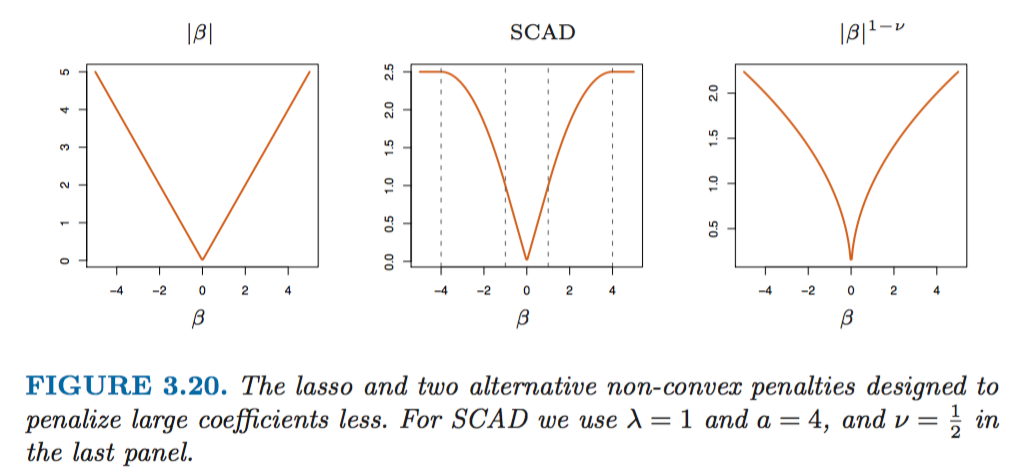
\includegraphics[width=4.5in]{./resources/lassopenalty}
\end{center}
\end{frame}



%%%%%%%%%%%%%%%%%%%%%%%%%%%%%%%%%%%%%%%%%%%%%%%%%%%%%%%%%%%%%%%%%%%%%%
\begin{frame}[allowframebreaks]
    \bibliographystyle{jpe}
    \bibliography{../empirical-methods}
\end{frame}

%%%%%%%%%%%%%%%%%%%%%%%%%%%%%%%%%%%%%%%%%%%%%%%%%%%%%%%%%%%%%%%%%%%%%%
\section*{Backup}
\subsection*{Info criteria}\label{sec:info}

\begin{frame}
    \frametitle{Review AIC/BIC}
    \begin{itemize}
    \item AIC tends to select larger models than BIC since it penalizes the number of parameters less heavily.
    \item These usually depend on ordering potential models by $p$ the number of components and then sequentially fitting them.
    \item AIC is not consistent: as $N \rightarrow \infty$ it may still select too many parameters.
    \item BIC is consistent: as $N \rightarrow \infty$ it will select the correct number of parameters.
    \item Of course for finite-sample $N < \infty$ anything can happen.
    \end{itemize}
\end{frame}
    
\begin{frame}
    \frametitle{Where does it come from?}
    How do we come up with these penalized regressions?
    \begin{itemize}
    \item AIC/BIC arise from considering the likelihood ratio test (LRT) of a maximum likelihood estimator and making a lot of assumptions.
    \item AIC arises from minimizing the Expected KLIC.
    \begin{eqnarray*}
    KLIC(f,g) &=& \int  f(y) \log(f(y)) \partial y - \int  f(y) \log(g(y)) \partial y  \\
    &=& C_f - E  \log(g(y))
    \end{eqnarray*}
    \item Low values of KLIC mean the models are similar.
    \end{itemize}
\end{frame}
    
\begin{frame}
    \frametitle{Where does it come from?}
    How do we come up with these penalized regressions?
    \begin{itemize}
    \item Recall that OLS is a ML estimator in the case where $\varepsilon$ is normally distributed.
    \begin{eqnarray*}
    D = - 2 \ln \left (\frac{\mbox{Likelihood  } H_0}{\mbox{ Likelihood  }H_a} \right) = -2 \ln \underbrace{\left(\frac{(\sup L(\theta | x) : \theta \in \Theta_0)}{(\sup L(\theta | x) : \theta \in \Theta)}\right)}_{\Lambda(x)}
    \end{eqnarray*}
    \item If the models are \alert{nested} then $\Theta_0 \subset \Theta$ and $\dim(\Theta) -\dim(\Theta_0) = q$ then as $N\rightarrow \infty$ we have that $D \rightarrow^d \chi^2(q)$.
    \end{itemize}
\end{frame}
    

\begin{frame}
\frametitle{Non-nested cases}
Many cases we are interested in are \alert{not strictly nested}
\begin{itemize}
\item Should I include $x_2$ OR $x_3$ in my regression? (partially overlapping)
\item Is the correct distribution $f(y | x, \theta)$ normal or log-normal? (non-overlapping)
\end{itemize}
\end{frame}

\begin{frame}
\frametitle{Non-nested cases}
\begin{itemize}
\item Cox (1961) suggested the following (often infeasible solution) by assuming that $F_{\theta}$ is the true model.
\begin{eqnarray*}
LR(\hat{\theta},\hat{\gamma}) = L_f(\hat{\theta}) - L_g (\hat{\gamma}) = \sum_{i=1}^N \ln \frac{f(y_i | x_i, \hat{\theta})}{g(y_i | x_i, \hat{\gamma})}
\end{eqnarray*}
\item Depending on which the true model is you could reject $F_{\theta}$ for $G_{\gamma}$ and vice versa!
\item Deriving the test statistic is hard (and specific to $F_{\theta}$) because we must obtain $E_f [\ln \frac{f(y_i | x_i, \hat{\theta})}{g(y_i | x_i, \hat{\gamma})}]$.
\item Similar to AIC in that we are minimizing KLIC over $F_{\theta}$.
\end{itemize}
\end{frame}

\begin{frame}
\frametitle{Vuong Test}
\begin{eqnarray*}
H_0: E_{h(y|x)} \left[ \frac{ f(y | x,\theta) }{g(y | x, \gamma)} \right] = 0  \\
\rightarrow E_h[\ln(h/g)] - E_h[\ln (h/f)] = 0
\end{eqnarray*}
\begin{itemize}
\item Instead of taking expectation with respect to one of two distributions, we take it with respect to $h(y |x)$ the unknown but \alert{true distribution}.
\item Same as testing whether two densities $(f,g)$ have same KLIC.
\item The main result is that (details in 8.5 of CT):
\begin{eqnarray*}
\frac{1}{\sqrt{N}} LR(\hat{\theta},\hat{\gamma}) \rightarrow^d N [0,\omega_{*}^2]\\
\omega_{*}^2 =  V_0 \left[ \ln \frac{f(y| x, \hat{\theta})}{g(y| x, \hat{\gamma})}  \right]
\end{eqnarray*}
\end{itemize}
\end{frame}


\begin{frame}
\frametitle{Non-nested cases}
Many cases we are interested in are \alert{not strictly nested}
\begin{itemize}
\item Should I include $x_2$ OR $x_3$ in my regression? (partially overlapping)
\item Is the correct distribution $f(y | x, \theta)$ normal or log-normal? (non-overlapping)
\end{itemize}
\end{frame}

\begin{frame}
\frametitle{Non-nested cases}
\begin{itemize}
\item Cox (1961) suggested the following (often infeasible solution) by assuming that $F_{\theta}$ is the true model.
\begin{eqnarray*}
LR(\hat{\theta},\hat{\gamma}) = L_f(\hat{\theta}) - L_g (\hat{\gamma}) = \sum_{i=1}^N \ln \frac{f(y_i | x_i, \hat{\theta})}{g(y_i | x_i, \hat{\gamma})}
\end{eqnarray*}
\item Depending on which the true model is you could reject $F_{\theta}$ for $G_{\gamma}$ and vice versa!
\item Deriving the test statistic is hard (and specific to $F_{\theta}$) because we must obtain $E_f [\ln \frac{f(y_i | x_i, \hat{\theta})}{g(y_i | x_i, \hat{\gamma})}]$.
\item Similar to AIC in that we are minimizing KLIC over $F_{\theta}$.
\end{itemize}
\end{frame}

\begin{frame}
\frametitle{Vuong Test}
\begin{eqnarray*}
H_0: E_{h(y|x)} \left[ \frac{ f(y | x,\theta) }{g(y | x, \gamma)} \right] = 0  \\
\rightarrow E_h[\ln(h/g)] - E_h[\ln (h/f)] = 0
\end{eqnarray*}
\begin{itemize}
\item Instead of taking expectation with respect to one of two distributions, we take it with respect to $h(y |x)$ the unknown but \alert{true distribution}.
\item Same as testing whether two densities $(f,g)$ have same KLIC.
\item The main result is that (details in 8.5 of CT):
\begin{eqnarray*}
\frac{1}{\sqrt{N}} LR(\hat{\theta},\hat{\gamma}) \rightarrow^d N [0,\omega_{*}^2]\\
\omega_{*}^2 =  V_0 \left[ \ln \frac{f(y| x, \hat{\theta})}{g(y| x, \hat{\gamma})}  \right]
\end{eqnarray*}
\end{itemize}
\end{frame}

\end{document}
